\chapter{Introduction}
\label{ch:introduction}
% %suggest some unity to two disparate projects.  
% Quantum mechanics is fundamentally a statistical theory, in that it only makes predictions for 
% the probabilities of events~\cite{Sakurai1994}.
% The probability for an event to occur is given by the Born rule, which says the probability is given by 
% the absolute-square of the probability amplitude for that event.  
% If there are multiple pathways by which an event can take place, the total amplitude for an event is 
% the sum over the amplitudes for each possible pathways~\cite{Feynman1965}.  
% These paths encompass paths through abstract spaces, such as the number of excitations in a field.
% In this case, the intermediate particles correspond to are referred to as ``virtual particles'', 
% which are referred to as quantum fluctuations.
% This sum over intermediate amplitudes can lead to novel quantum effects such as the Casimir effect,
% where electrically neutral, material bodies are attracted to each other due to the exchange of virtual photons.
% %\comment{Perhaps Peres?}

% Alternatively, the probabilistic nature of quantum mechanics implies that the results of quantum measurements 
% are stochastic quantities which fluctuate under repeated measurements.  
% This is particularly relevant as modern experiments can isolate single quantum systems for long 
% periods of time and continuously measure their properties.  One can then think of reconstructing
% the system's trajectory through time as it evolves based on the measurement~\cite{Carmichael1993}.  

% This thesis presents two projects reflecting each aspect of quantum fluctuations.  
% The projects are further connected by their quantum mechanical underpinning, the computational methods 
% employed to simulate stochastic processes, and their relevance to modern experiments on atoms.  
% The first project is a method of computing energies related to Casimir effect, while the second project is related to 
% continuous quantum position measurements of atoms.  The majority of this thesis will be devoted
% to the first project, with the second project being discussed in the final chapter.  
% The key results presented in this thesis have been published in~\cite{
% Mackrory2010, Mackrory2016,Mackrory2017a, Mackrory2017b}
% % Through advances in modern experimental technology both of these categories of effect are now 
% % directly observable.%~\cite{WisemanMilburn2010, Dalvit2011}.  

% % The first project relates to computing Casimir forces via the worldline method, and occupies the majority
% % of this thesis.  In brief, the worldline method is a Monte Carlo method for computing Casimir energies
% % via ensembles of closed Brownian paths.  The work presented here extends the method by
% %  developing analytical and numerical techniques to 

% % The second theme will be using quantum trajectories to simulate continuous positions measurements on atoms.
% % Both of these projects are related to fundamental quantum optical phenomena, 
% % that we will explore using stochastic calculus, and Monte-Carlo methods for numerical simulations.  

% The remainder of the introduction will expand on the physical origin, modern experiments, and theoretical
% techniques for computing both Casimir effects, and then continuous quantum measurements.  

% % \comment{There are two roles for the randomness here.
% %   From one point of view, the randomness is an intrinsic part of quantum mechanics,
% %  and thus naturally shows up in fluctuation phenomena like the Casimir effect, or in quantum measurements.
% %   Alternatively, if we are considering these calculations for energy or evolution as large integrals,
% %  then we can efficiently compute these integrals by randomly sampling from their dominant regions.
% %   In this sense, the randomness shows up as a calculational tool.}

% % \begin{enumerate}
% % \item General thesis about quantum physics of atoms using computation.  
% % \item Thesis covers numerical monte-carlo techniques, where random numbers used in simulation.
% % \item First new method for computing electromagnetic Casimir energies.
% % \item Second, continuous position measurements of atoms taking into account experimental constraints.  
% % \item United in perspective of numerical work relying on Monte-Carlo techniques,
% %  to explore quantum phenomena relevant to modern experiments and pushes toward future technology  
% % \end{enumerate}

%\section{Casimir Forces}% in general and physical interpretation}

The Casimir force is a striking manifestation of quantum field theory: a pair of electrically neutral,
 conducting bodies will be attracted to one another due to their interaction
with quantized electromagnetic fields, even in the absence of photons~\cite{Casimir1948}.  
% The Casimir force is a primarily attractive force that arises between material bodies interacting via 
% quantized fields~\cite{Casimir1948}.
While the Casimir effect is a generic consequence of quantum field theory subject to boundary conditions,
the most important example is due to fluctuations in the electromagnetic (EM) field.  The quanta of the 
EM field, photons, are massless making their interaction long-ranged, and their coupling to matter is much stronger
than the other long-ranged fundamental force, gravity.  
In the electromagnetic Casimir effect, one can think of the electrons in a body emitting and absorbing virtual photons that can in turn
interact with electrons in other bodies.  The interacting bodies can be pairs of atoms~\cite{CasimirPolder1948}, 
macroscopic bodies such as metallic planes and dielectric slabs~\cite{Lifshitz1956}, or any combination of these.

Alternatively, the Casimir effect can be attributed to the attraction between instantaneous dipoles forming in the bodies.  
This interpretation is intimately related to the van der Waals force, where 
molecules with fluctuating dipole moments are attracted to one another~\cite{vanderWaals}.
While the emphasis may differ between Casimir and van der Waals forces, they ultimately describe the 
same phenomenon, albeit at slightly different distance scales.  

Despite the prediction of the Casimir force in 1948, precise measurements of the Casimir force were only
carried out in the late 1990s~\cite{Lamoreaux1997,Mohideen1998}.  Early attempts failed due to the difficulty
in aligning parallel conducting plates (as in Casimir's first calculation), while these experiments used a
sphere above a conducting plate.  Experiments have also been
carried out to measure the forces between atoms and surfaces~\cite{Sukenik1993,Perreault2005,Harber2005}.

Beyond their importance as manifestations of quantum field theory, Casimir effects are also 
important to a range of modern experiments and developing technologies.
They are important for microelectromechanical systems (MEMS) where the Casimir attraction between components 
leads to stiction, where pieces are permanently stuck together~\cite{Buks2001}.  
Casimir forces are also important for developing technologies using atoms near dielectric surfaces~\cite{Folman2000,Alton2011, Hung2013}.
In these experiments, the attractive Casimir potential sets a lower bound for how
close the atoms can be brought to the surface, and as a result must be considered in the engineering 
of these devices.

The advent of these experiments in complicated arrangements of bodies, has spurred the development
of a number of theoretical and computational methods for computing Casimir~\cite{Dalvit2011,Bordag2009}. 
To model these experiments, it is necessary to be able to compute the Casimir effect between arbitrarily shaped bodies, with 
realistic material properties --- this in general necessitates a numerical approach~\cite{Johnson2011}.
The most important of these modern methods are the so-called ``scattering method''~\cite{Lambrecht2006,Rahi2009,Reid2009}
 and ``worldline methods''~\cite{Gies2003}.

To date, the scattering method is the only general purpose numerical method available for computing
Casimir forces in arbitrary arrangements of bodies~\cite{Reid2009,Reid2011,Reid2013}.  
In this method, one considers fluctuating currents confined to the surfaces of the interacting bodies,
where the currents at each patch of surface interact with one another via the appropriate EM Green functions,
which can be thought of as photons.  One finds the Casimir energy by taking the determinant 
of the (large) scattering matrix for all of these patches~\cite{Reid2011}.  

The worldline method is a promising alternative method for computing Casimir energies~\cite{Gies2003}.  
The worldline method computes the Casimir energy by considering an ensemble of closed 
Brownian paths propagating through space.  The presence of bodies is encoded in a potential which is
accumulated along the path based on whether the Brownian paths intersect any of the bodies.  One can
intuitively consider these paths as being the space-time path of a virtual particle.  
The worldline method has only been developed for scalar fields interacting with idealized surfaces.
In contrast to the scattering method, the worldline method is a Monte Carlo method which makes it 
easy to parallelize.  

It is the goal of this thesis to extend the worldline method to computing electromagnetic Casimir effects.
This requires accounting for the vector nature of the EM field, and including realistic coupling to 
material properties, while attempting to retain as many of its appealing
properties as possible.    

The rest of this introduction will cover simple examples of Casimir effects, and expand background material.
In Sec.~\ref{sec:Casimir}, we will introduce some simple calculations for Casimir effects such as
the Casimir--Polder potential between an atom and a conducting wall, and the Lifshitz formula for the Casimir
effect between dielectric half-spaces (both of which we will use as checks on our later work).
We will then briefly discuss relevant experiments in Sec.~\ref{sec:experiments}, and expand on our discussion
of the numerical methods in Sec.~\ref{sec:numerical_review}.  

% At the outset, we note that there have been a number of books published on the subject of Casimir forces 
% in recent years.  This reflects the importance of Casimir forces to both physicists and chemists, as 
% well as the advent of new experiments which have spurred the development of new theoretical methods.  
% Milonni's clear text on QED sets the Casimir force in context as one manifestation of the quantized theory of light~\cite{Milonni1994}.
% while Milton's text emphasizes using Green function methods for computing a number of consequences for 
% the Casimir effect for various fields, dimensions~\cite{Milton2001}.
% There have been more recent where the state-of-the-art in both theory and experiments is discussed by practitioners --- 
% notably in the volumes by Bordag~\etal\cite{Bordag2009}, 
% and the collection editted by Dalvit~\etal\cite{Dalvit2011}.  
%\todo{Cite Vogel and Welsch~\cite{VogelWelsch2006}.  Also cite Buhmann~\cite{Buhmann2012-vol1,Buhmann2012-vol2}}
% While this thesis emphasizes simple physical applications, the application of Casimir or 
% van der Waals forces is also important to problems in surface physics and chemistry, as discussed in the texts by 
%  Parsegian~\cite{Parsegian2006} and Israelachivili~\etal~\cite{Israelachvili2011}.

% The references in the following sections are given to emphasize the important results and calculations
% and set the basic context for Casimir effects.   In addition we will often use these results 
% as checks in our later work.  % Broader bibliographic surveys of the (vast) Casimir literature
% % are available from Milton~\cite{Milton-bib} and Babb~\cite{Babb-bib}.

\section{Casimir Effect}

As alluded to earlier, Casimir and van der Waals forces are one and the same.  The Casimir
interpretation ascribes the interaction to fluctuations in the electromagnetic field, while van der 
Waals forces are ascribed to the molecular dipoles.  
Historically, van der Waals found deviations from ideal gas behaviour, which can be attributed 
to the atoms possessing a finite size and being attracted to one another~\cite{vanderWaals,Parsegian2006}.
%(A fuller account of the scientific history of these forces is discussed in Parsegian~\cite{Parsegian2006}.)
While a number of different inter-molecular forces due to permanant
 or fluctuating electric dipoles are possible~\cite{Israelachvili2011},
we are primarily interested in forces due to fluctuating dipoles.  
These molecular dispersion forces are typically referred to as London forces after London's work
 using quantum mechanical perturbation theory to compute the potential between atoms~\cite{London1930}.  
The potential has a characteristic $d^{-6}$ scaling.  

However, the Casimir effect was framed in the more modern language of quantum field theory, 
which more naturally encompasses van der Waals forces between molecules.  
Furthermore, Casimir and Polder computed the potential between molecules 
using quantum field theory to account for retardation effects, and leads to a richer range of phenomena~\cite{CasimirPolder1948}.  
As a result, we start our discussion with their work.  

\subsection{Casimir--Polder Forces}

In 1948 Casimir and Polder extended this theory to using Quantum Electrodynamics
(QED) to account for the retardation due to the finite speed of light~\cite{CasimirPolder1948}. 
They found that in the far-field 
(where the transition wavelengths $c/\omega_A$ exceed the separation of the atoms $d$, $d\gg c/\omega_A$)
the interatomic potential decays more rapidly as $d^{-7}$.  The change in power law can be 
attributed to the induced dipoles decorrelating over the time-of-flight of the virtual photon, 
and thus having a weaker interaction.  
\todo{Is this from Milonni?}
Furthermore, they found an attractive force between an atom and perfectly conducting wall, with a $d^{-3}$ scaling
in the near field (van der Waals) regime, passes over to $d^{-4}$ scaling in the far-field.
In this case the atom can be thought of as interacting with it's image in the perfect conductor,   
which leads to an attractive potential for the atom,
\begin{equation}
  V_{CP}(d) =-\frac{3\hbar c\alpha_0}{64\pi^2\epsilon_0 d^4},
\end{equation}
where $\hbar$ is the reduced Planck's constant, $c$ is the speed of light, $\alpha_0$ is the atom's static polarizability,
and $\epsilon_0$ is the permittivity of free space.  Throughout this thesis we will refer to these
atom-wall type forces as Casimir-Polder forces.  

\subsubsection{Derivation of the Atom-Perfect Conductor potential}
\label{sec:CP_calc}
The Casimir--Polder potential between an atom in its ground state and a surface can be derived via perturbation theory
in the coupling of the atom to the electromagnetic field.  
(This derivation is adapted from Ch.~13 and \S14.3 of Steck~\cite{SteckNotes}.)
The Hamiltonian for the whole atom-field system is given by 
\begin{equation}
  H = H_{\text{atom}} + H_{\text{field}} + H_{\text{int}}
\end{equation}
where 
\begin{gather}
  H_{\text{atom}} = \frac{\hat{\vect{p}}^2}{2m} + \sum_j\hbar\omega_{j}\sigma_j^\dag\sigma_j  \\
  H_{\text{field}} = \sum\subkz \hbar\omega_k\left(a^\dag\subkz a\subkz + \frac{1}{2}\right)\\
  H_{\text{int}} = -\vect{d\cdot E} = \sum_j\sum\subkz
  \sqrt{\frac{\hbar\omega_k}{2\epsilon_0}}(\sigma_j+\sigma_j^\dag)
  \vect{d}_j[a\subkz \vect{f}^*_k(\hat{x})+a^\dag\subkz \vect{f}\subkz(\hat{x})]
\end{gather}
The atomic Hamiltonian $H_{\text{atom}}$ is split into a center-of-mass piece, and the internal degrees of freedom,
described by the atom's quantized energy levels with energy $E_j=\hbar\omega_j$, 
and $\sigma_j=|g\rangle\langle e_j|$ is the lowering operator for the atom's internal state.  
The field Hamiltonian sums up the energy for each mode of the electromagnetic field and 
includes the zero-point energy, $\sum_k\hbar\omega_k/2$.
For the Casimir--Polder calculation, this zero-point-energy is a divergent constant which drops out when
considering the energy differences when the atom is moved to spatial infinity.  
The interaction Hamiltonian couples the internal state of the atom to the quantized light field,
where $a\subkz$ is the annihilation operator for mode with wavenumber $k$, and polarization $\zeta$,
which has spatial mode function $\vect{f}\subkz(\hat{x}).$
In this calculation the mode functions $\vect{f}\subkz$ must satisfy the electromagnetic boundary conditions
on the surfaces of the bodies.  The resulting electromagnetic mode functions (and thus the potential)
are then sensitive to the arrangements of the bodies.  
%This is distinct from the case in most field theory calculations where the modes are described by plane waves.  

Note that some of the terms in the interaction Hamiltonian violate energy conservation, for example
$\sigma_j^\dag a^\dag\subkz$ creates a photon and raises the atom from the ground state to an excited state.
These terms are normally dropped in the rotating-wave-approximation, since they oscillate quickly
in time as $e^{-i(\omega_j+\omega_k)t}$, and average down to zero on typical atomic timescales.  
However, these energy non-conserving terms do lead to observable effects at higher order in perturbation theory.
% This theory treats the interaction of the atoms with the light field via the interaction Hamiltonian
% \begin{equation}
%   H_{\text{int}} = -\frac{e}{mc}\hat{\vect{p}}\cdot\hat{\vect{A}}(\hat{\vect{x}}) + \frac{e^2}{2mc^2}
%   |\hat{\vect{A}}(\hat{\vect{x}})|^2
% \end{equation}
% where $\hat{\vect{p}}$ is the quantum momentum operator for the atom, and $\hat{\vect{A}}$ is the 
% quantized operator for the EM vector potential at the atom's position $\vect{r}$.  \todo{Expand field operators
% $\op{A}(\vect{x},t) = \sum_k a_k e^{-i\omega_k t} f_k(\vect{x}) + \text{h.c}$}
% (This interaction can instead be treated with $H_{\text{int}} = -\op{\vect{d}}\cdot \op{\vect{E}}$ where
% these Hamiltonians are connected by the Power-Zienau transformation~\cite{SteckNotes}.\todo{Find page})
In particular, the Casimir--Polder potential emerges when computing the energy-shift from $H_{\text{int}}$ to second order.
For an atom in it's ground state, the Casimir--Polder potential is given by
\begin{equation}
  V\subCP = -\sum_{n\ne 0,\vect{k},\zeta} \frac{
    \langle E_0, 0|  H_{\text{int}}|E_n, 1\subkz\rangle\langle E_n, 1\subkz|  H_{\text{int}}|E_0, 0\rangle}{\hbar(\omega_k+\omega_{n0})},
\end{equation}
where $|E_n,1\subkz\rangle$ denotes the state with the atom in energy level $n$ and one photon in mode $\vect{k}$,
$|0\rangle$ denotes the vacuum state of the electromagnetic field, and the transition frequency $\omega_{n0}=(E_n-E_0)\hbar$.
The shift $V\subCP$ can be understood as two virtual transitions --- one from the ground state with no photons to an excited state with one photon,
and then a return transition.  The total energy shift is found by summing over all possible intermediate states.
This process is represented schematically via the Feynman diagram in Fig.~\ref{fig:feynman_CP}, where 
an atom in the ground-state emits a virtual photon, and re-absorbs it.  This transition
is a ``virtual'' one, since these intermediate states are not directly physically observable on a detector
%, % but rather reflect the apparatus of quantum mechanical perturbation theory
.
\begin{figure}
  \centering
\begin{fmffile}{atom-loop}
  \begin{fmfgraph*}(60,30)
    \fmfleft{i}
    \fmfright{o}
    \fmftop{t}
    \fmf{plain}{i,v1}
    \fmf{plain}{v2,o}
    \fmf{plain,label=$|e_j\rangle$}{v1,v2}
    \fmf{photon,left=0.5,tension=.4}{v1,vt,v2}
    \fmf{phantom,tension=1}{t,vt}
    \fmflabel{$|g\rangle$}{i}
    \fmflabel{$|g\rangle$}{o}
    \fmflabel{$|1_{\vect{k}}\rangle$}{vt}
  \end{fmfgraph*}
\end{fmffile}
\caption[Feynman Diagram for Casimir-Polder Energy]
{Feynman diagram representing an atom interacting with electromagnetic field via emitting and absorbing photons.  
  The wavy line represents the electromagnetic Green function in the presence of boundaries --- as opposed to the usual plane 
  waves exploiting in field theory computations.  The atom is excited into intermediate states.
}
\label{fig:feynman_CP}
\end{figure}
% \comment{This is rote copying of Dan's notes - pointless!}

% while the EM Green function is 
% \begin{equation}
%   G_{ij}(\vect{r},\vect{r'},\omega) = \sum\subkz \omega_k
%   \frac{f_{\vect{k},\zeta,i}(\vect{r})f^*_{\vect{k},\zeta,j}(\vect{r'})}{\omega_k^2-\omega^2}.
% \end{equation}
% which satisfies
% \begin{equation}
%   \nabla\times\nabla\times G(\vect{x},\vect{x'}) 
%   + \frac{\omega^2}{c^2}\epsilon G(\vect{x},\vect{x'}) 
%   = \omega^2\delta_{ij}\delta(\vect{x-x'}).
% \end{equation}

After substituting in $H_{\text{int}}$, the Casimir--Polder energy can be written as
\begin{align}
  V\subCP(\vect{r}) % &= -\sum_{m\ne 0,\vect{k},\zeta} \frac{
    % \langle E_g, 0|d_if_{\vect{k},\zeta,i}a\subkz|E_n, 1\subkz\rangle
    % \langle E_n, 1\subkz|d_jf^*_{\vect{k},\zeta,i}a^\dag\subkz|E_g, 0\rangle}{\hbar(\omega_k+\omega_{n0})}\\
% &= -\sum_{m\ne n,\vect{k},\zeta} \frac{\hbar\omega_k}{2\epsilon_0}
%     \frac{\langle E_0|d_i|E_n\rangle \langle E_n|d_j|E_0\rangle f_{\vect{k},\zeta,i}(\vect{r})f^*_{\vect{k},\zeta,j}(\vect{r})
%     }{\hbar(\omega_k+\omega_{n0})},\\
&= -\sum_{m\ne 0,\vect{k},\zeta} \frac{\hbar\omega_k}{6\epsilon_0}
    \frac{|\langle E_0|\vect{d}|E_n\rangle|^2 |\vect{f}_{\vect{k},\zeta,i}(\vect{r})|^2}
    {\hbar(\omega_k+\omega_{n0})},
\end{align}
where we substituted the form of $H_{\text{int}}$ and assumed an spherical atom for which all components of dipole matrix elements
are equal, such that $|\langle E_0|d_i|E_n\rangle|^2=|\langle E_0|\vect{d}|E_n\rangle|^2/3$.

The Casimir--Polder potential can now be factored into atomic and field pieces~\cite{McLachlan1963}.
The first is the polarizability for the atom in its ground state is
\begin{equation}
  \alpha_{ij}(\omega) = \sum_n 
  \frac{2\omega_{n0}\langle E_0|d_i|E_n\rangle\langle E_n| d_j|E_0\rangle}{\hbar(\omega_{n0}^2-\omega^2)},
\end{equation}
is the susceptibility of the atom to perturbations in the electric field.

If we assume the atom's distance from the surface $d$ is larger than the atom's dominant emission wavelength,
then the dominant contribution to the sum will come from frequencies for which $\omega_kd/c\sim 1$.
$\omega_k\ll \omega_{n0}$.  
The atomic polarizability can be replaced by the atom's static (zero frequency) polarizability 
\begin{equation}
  \lim_{\omega\rightarrow 0}\alpha(\omega) = \sum_n
  \frac{2|\langle E_0|\vect{d}|E_n\rangle|^2}{3\hbar\omega_{n0}},
\end{equation}
In this far-field limit, the Casimir--Polder energy can be approximated as 
\begin{equation}
  V_{CP}(\vect{r})= -\frac{\hbar}{4\epsilon_0}\alpha_0\sum_{\vect{k},\zeta}\omega_k |\vect{f}_{\vect{k},\zeta,i}(\vect{r})|^2
\end{equation}

At this point, the mode functions for the electric field near a perfectly conducting plane 
can be substituted in to the energy.  (\S 8.4.3 of Steck~\cite{SteckNotes}),
or mode functions for a perfectly conducting box(\S3.12 in Milonni~\cite{Milonni1994}).
The electromagnetic mode functions for perfectly conducting box are given by 
\begin{align}
  \vect{f}\subkz(\vect{r}) = \sqrt{\frac{8}{V}}\bigg[&
  \hat{x}(\hat{\varepsilon}\subkz\cdot\hat{x})\cos(k_xx)\sin(k_y y)\sin(k_zz)\nonumber\\
  &+\hat{y}(\hat{\varepsilon}\subkz\cdot\hat{y})\sin(k_xx)\cos(k_y y)\sin(k_zz)\nonumber\\
  &+\hat{z}(\hat{\varepsilon}\subkz\cdot\hat{z})\sin(k_xx)\sin(k_y y)\cos(k_zz)\bigg],
\end{align}
where $\hat{\varepsilon}\subkz$ are the polarization unit vectors, and the wavenumbers $k_i=n_i\pi/L$,
with $n_i$ integers~(\S 8.4.1 of Steck~\cite{SteckNotes}).
% The Casimir--Polder energy for an atom and a perfectly conducting wall is then 
% \begin{align}
%  V\subCP(\vect{r})=-\frac{2\hbar}{\epsilon_0V}\alpha_0\sum_{\vect{k},\zeta} \big[ &
%   (\hat{\varepsilon}\subkz\cdot\hat{x})^2\cos^2(k_xx)\sin^2(k_y y)\sin^2(k_zz)\nonumber\\
%   &+(\hat{\varepsilon}\subkz\cdot\hat{y})^2\sin^2(k_xx)\cos^2(k_y y)\sin^2(k_zz)\nonumber\\
%   &+(\hat{\varepsilon}\subkz\cdot\hat{z})^2\sin^2(k_xx)\sin^2(k_y y)\cos^2(k_zz)\bigg].
% \end{align}
If we assume that the atom is close to the $z=0$ plane, but far from the other walls, the $x,y$ sinusoids
can be replaced by their average value of a half, since they will be quickly oscillating.   
In addition, the polarization vectors form a resolution of the transverse identity (since Gauss's law 
implies that the electric field is transverse, $\nabla\cdot\vect{E}=0$),
\begin{equation}
  \sum_{\zeta} \hat{\varepsilon}\subkz^{i}\hat{\varepsilon}\subkz^{j} = \delta_{ij}-\frac{k_ik_j}{k^2}.
\end{equation}
With these simplifications, and taking the limit of a large box to convert the sum over wavevectors into an
integral, the Casimir--Polder potential is given by 
\begin{align}
 V\subCP(\vect{r})=-\frac{\hbar\alpha_0}{8\pi^3\epsilon_0}\int d^3k\,\omega_k\bigg[ &
  \bigg(1-\frac{k_x^2}{k^2}\bigg)[1-\cos(2k_zz)]
  +\bigg(1-\frac{k_y^2}{k^2}\bigg)[1-\cos(2k_zz)]\nonumber\\
  &+\bigg(1-\frac{k_z^2}{k^2}\bigg)[1+\cos(2k_z z)]\bigg]
\end{align}
where we have rewritten the sinusoids using double-angle formulae.  The $z$-independent parts
lead to a constant, divergent contribution to the energy.  
In order to extract a finite energy shift it is essential to renormalize the energy by subtracting
off this constant energy.  This corresponds to considering the energy change as the atom is brought
close to the surface from spatial infinity.  
Throughout this thesis, this simple energy subtraction is the only renormalization we will need. 

The renormalized Casimir--Polder energy for an atom-conducting-plane can be evaluated in spherical
coordinates, although some care is required to regularize these oscillatory integrals --- this can be done by introducing an exponential
convergence factor $e^{-a k}$ and taking the limit $a\rightarrow 0$ at the end of the computation,
\begin{align}
 V\subCP(\vect{r})- V\sup0&=\lim_{a\rightarrow 0}-\frac{\hbar\alpha_0}{8\pi^3\epsilon_0}\int d^3k\,\omega_k 
  (-1)\frac{2k_z^2}{k^2}\cos(2k_zz) e^{-ka}\\
&=\lim_{a\rightarrow 0}\frac{\hbar c\alpha_0}{4\pi^2\epsilon_0}\int_0^\infty dk \int_0^\pi d\theta\,k^3\sin\theta 
  \cos^2\theta\cos(2kz\cos\theta) e^{-ka}\\
&=-\frac{\hbar c\alpha_0}{4\pi^2\epsilon_0}\frac{3}{2z^4}.
\end{align}
While we have emphasized the case of perfectly-conducting planar interfaces, similar computations
can be carried out for dielectric interfaces and more general shapes of macroscopic bodies.  
However, this type of calculation relies on having analytical expressions available for the mode functions,
which limits this approach to highly symmetric geometries.  

% The Casimir--Polder energy can be further factored in terms of atomic polarizabilities,
% and Green functions for the electromagnetic field~\cite{McLachlan1963}. 
% The atomic polarizability measures the linear response of an atom to the electromagnetic field,
% and is given by 
% where $d_i$ is the $i^\text{th}$ component of the dipole operator $\vect{d}=e\vect{r}$.
% \todo{What does polarizability look like for a simple atom?}
% At this order of perturbation theory, the EM Green tensor is given by its classical counterpart,

% To linear order in the coupling, the energy can be written on the imaginary frequency $is$ as 
% \begin{equation}
%   V\subCP(\vect{x}) = -\frac{\hbar c}{2}\int_0^\infty ds \alpha_{jk}(is)G^{(S)}_{kj}(\vect{r},\vect{r},is),
% \end{equation}
% where $\alpha_{ij}$ is the polarizability tensor, $G^{(S)}$ is the scattering part of the EM Green
% tensor~\cite{McLachlan1963, McLachlan1963a}.
% The scattering part of the Green function essentially subtracts off the vacuum 
% EM Green function $G^{(S)}=G-G^{(0)}$ --- this is essentially renormalizing the energy
% by subtracting off contributions that are independent of the bodies.  
% This has the same from as a linear-response calculation~\cite{Altland2011}, finding the linear-response of the 
% atom to it's interaction with the EM field.

% While we have only given the linear energy shift, there are a number of higher loop contributions
% which can be resummed analytically due to the relative simplicity of the expansion~\cite{Rosa2011}.  
% \todo{Cite Dzyaloshinksii or papers book for resummation?}
% The result of which is 
% \begin{equation}
%   V\subCP(\vect{r}) = \frac{\hbar c}{2\pi}\int_0^\infty ds \tr \log[I - \alpha(is) G^{(S)}(\vect{r},\vect{r})].
% \end{equation}
% This method of computing Casimir--Polder energies via classical Green functions has been expanded upon
% in Ch. 7 of Milonni~\cite{Milonni1994}, Vogel and Welsch~\cite{VogelWelsch2006} and Buhmann~\cite{Buhmann2012-vol1,Buhmann2012-vol2}.

% \begin{enumerate}
% %\item Cite Lifshitz, Dzyaloshinski, Abrisokov.
% \item Cite Schwinger~\cite{Schwinger1978, Milton1978}  Scalar green functions.  
% \item Green tensor methods
% \item Cite Barton
% \end{enumerate}

\subsection{Forces between bodies: Casimir Energy}

The classic example due to Casimir~\cite{Casimir1948} predicts that a pair of electrically neutral,
perfectly conducting plates will attract one another due to their interaction with the quantized 
electromagnetic (EM) field.  
The presence of the conductors forces the electric field to vanish on the surfaces,
which restricts the allowed modes of the electromagnetic field, as illustrated in Fig.~\ref{fig:Casimir_sketch}.
Each quantized mode of the electromagnetic field contributes
to the energy, even in the ground state with zero photons.  Each mode contributes 
$E_\alpha=\hbar\omega_\alpha/2$ , where $\hbar$ is Planck's  constant, and $\omega_\alpha$ is the frequency of the mode.
The total energy is found by summing the mode for each energy --- the total energy is
badly divergent since each term in the sum is positive.  However a finite answer can 
be found by consider an energy \emph{difference} between two different configurations.  
The subtraction to eliminate divergences is a simple form of field theoretic renormalization, 
and will be essential in computations of Casimir quantities.  
In this case, the energy when the bodies are removed to spatial infinity is subtracted.  
The renormalized energy between the plates is
\begin{equation}
  E-E_0 = -\frac{\hbar c}{240\pi^2 d^3},
\end{equation}
where $c$ is the speed of light in vacuum, $\hbar$ is the reduced Planck constant,
and $d$ is the distance between the plates.  Note that in this expression there is no
mention of the material properties of the media --- this is an artifact of imposing Dirichlet
boundary conditions on the surfaces.  

\begin{figure}
\center
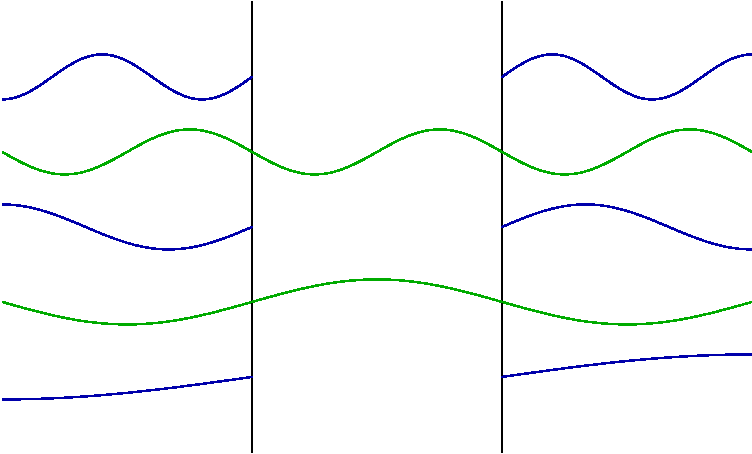
\includegraphics[width=6cm]{fig/intro/twoplanes_wave}
\caption[Allowed modes between parallel plates]
{Sketch of allowed modes between perfectly conducting plates. 
 Only waves with a half-integer number of wavelengths fit between the plates.
Blue modes are only allowed outside the plates, while green modes are allowed inside
and outside.  Modes have been vertically offset for clarity.  }
\label{fig:Casimir_sketch}
\end{figure}

The theory was extended by Lifshitz to describe forces between dielectric half-spaces~\cite{Lifshitz1956,
Dzyaloshinskii1959,Dzyaloshinskii1961}.  This can recover the Casimir force between 
perfect conductors, and Casimir--Polder forces between atoms' and dielectric surfaces.  
%  As intimidating as this expression is, it can be heuristically derived with
% relative ease via the ``argument principle''~\cite{vanKampen1968}.  
% In essence, since the Casimir energy is the sum of the vacuum energy over all modes, the energy can
% be written as a complex contour integral of the energy against a function with poles at the allowed 
% energies.  For two plates the allowed modes satisfy the Fabry-Perot condition,
% \begin{equation}
%   \Delta = 1 - r_1r_2 e^{2ik d}.
% \end{equation}

It is often convenient for calculations to write the energy in terms of the imaginary frequency, $\omega = -is$,
since for causal functions (such as an atom's or dielectric's response to the electromagnetic field), 
the response is analytic on the imaginary axis.    \todo{Cite Johnson for benefits?  Kramers-Kr\"onig relations.}
This procedure avoids the poles along the real-frequency axis, and instead replaces oscillatory
integrals with smoothly decaying real functions, that are much more amenable to numerical studies~\cite{Johnson2011}.

\subsubsection{Derivation of Lifshitz Formula}

The energy for the EM field in its ground state is 
\begin{equation}
  E = \sum_{\zeta}\sum_{k_x,k_y,\omega} \frac{\hbar\omega_k}{2},
\end{equation}
where the sum runs over all of the allowed modes for the particular arrangement of bodies.  
The Casimir energy can be found with an ingenious argument due to van Kampen~\etal
~\cite{vanKampen1968}.  (Our treatment parallels \S 7.2 in Milonni~\cite{Milonni1994}.)
The sum over frequencies can be recast as a contour integral over a function whose poles occur at the allowed
frequencies, with residue $\omega_k$:  
\begin{equation}
  E = \frac{L^2}{(2\pi)^2}\int_0^\infty dk_T\,k_T\oint d\xi\, \frac{\hbar \xi}{2} \frac{1}{(2\pi i)\Delta(\xi)}\frac{d\Delta(\xi)}{d\xi},
\end{equation}
where the function $\Delta'(\xi)/[2\pi i\Delta(\xi)]$ is designed to have unit residue at the zeroes of $\Delta(\xi)$, 
and $k_T$ is the transverse wavenumber.  
The energy can be simplified by integrating by parts leading to 
\begin{equation}
  E = \frac{\hbar}{16\pi^3 i}\int d^2k_Tk_T\oint d\xi \, \ln\Delta(\xi).
\end{equation}
The most important modes are the surface modes, since these modes are sensitive to the position of the other body, where
these modes exponentially decay between the bodies.    The allowed frequencies for these modes must 
satisfy 
\begin{equation}
  r^{\zeta}_1r^{\zeta}_2 e^{-2k_z d}=1,
\end{equation}
where $r^\zeta_i$ are the reflection coefficients for surface $i$ and polarization $\zeta$.
This is suggestive of the requirement that accumulated round-trip phase (including reflections from both walls) is unity for
allowed modes.  (This interpretation is bolstered by examining the Casimir force between mirrors~\cite{Genet2003}.)
This suggests choosing $\Delta(\xi) = 1-r^{\zeta}_1r^{\zeta}_2 e^{-2k_z d}$, where the wavenumber $k_z$
and the reflection coefficients are functions of $\xi$.  


%\begin{itemize}
  % \item $E = \sum_k\frac{\hbar \omega_k}{2}$
  % \item Should insert sum over transverse momenta.  This sum runs over all modes, not just frequency.
  % \item Only allowed modes contribute.  
    % Between two plates, the allowed modes must satisfy the Fabry-Perot criterion: 
    % $\Delta = 1- r_1r_2e^{2ik_3d} =0$.
  % \item Use fact that in complex analysis integrating function in closed loop in complex plane gets
  %   $\oint dz f(z) = 2\pi i\sum_{\text{poles} z_i}\text{Res} f(z_i)$.
  % \item So energy can be written as 
  %   \begin{equation}
  %     E = \sum_k \frac{\hbar \omega_k}{2} = \oint dz \frac{\hbar z}{2(2\pi i)} \frac{\Delta'(z)}{\Delta(z)},
  %   \end{equation}

  % \item Now integrate by parts w.r.t. $z$
  %   \begin{equation}
  %     E = \oint dz \frac{\hbar}{2(2\pi i)} \log\Delta(z).
  %   \end{equation}
  % \item Now differentiate w.r.t $d$ to get force, and done.  
%\end{itemize}

The Casimir energy between two dielectric half-spaces of permittivities $\epsilon_1,\epsilon_2$
separated by a gap of thickness filled with permittivity $\epsilon_3$ is given by 
\begin{align}
\frac{E}{L^2} =& -\frac{\hbar}{2\pi^2c^3}\int_0^\infty d\xi \xi^2 \epsilon_3
\int_1^\infty dp\,p\sum_{\zeta=\text{TE, TM}}\log\left[1 - r^{(\zeta)}_{13}r^{(\zeta)}_{23}e^{-2\sqrt{\epsilon_3}p\xi d/c}\right]
\end{align}
where the electromagnetic reflection coefficients are given by 
\begin{align}
  r\supTE_{ij}  = \frac{s_i-s_j}{s_i+s_j},\quad
  r\supTM_{ij}  = \frac{\epsilon_j s_i - \epsilon_i s_j}{\epsilon_j s_i + \epsilon_i s_j},
\end{align}
and
\begin{equation}
  s_i = \sqrt{p^2 + \epsilon_i/\epsilon_3-1}
\end{equation}
following Zhou~\cite{Zhou1995}. 

% This was further expanded on by Dzyaloshinskii~\etal\cite{Dzyaloshinskii1959,Dzyaloshinskii1961} who
% showed the connection between Casimir force and the pair-wise van der Waals potentials.  
%This work is reviewed by McLachlan~\cite{McLachlan1963, McLachlan1963a}.  

The Casimir--Polder results for interacting atoms are recovered from the Lifshitz formula by taking the limit of dilute bodies,
$\epsilon \approx 1+\alpha n$, where $n\ll 1$ is the density, and $\alpha$ is the polarizability.
In addition, the perfect-conductor Casimir can be found by taking $r_i\rightarrow 1$, and evaluating the 
integrals.

The Lifshitz theory can be extended to account for dispersion and finite temperature.  
Some care is required in quantizing the electromagnetic field within dielectric media,
since due to the Kramers-Kr\"onig relations, the presence of dispersion implies dissipation.
The usual approach to open-systems in quantum mechanics is to couple the system to a reservoir, 
and then trace out, or integrate out, the reservoir.
It has been phenomenologically observed that one gets the correct answers by a direct substitution
$\epsilon(\vect{x})\rightarrow \epsilon(\omega,\vect{x})$.  This issue has in investigated in~
\cite{Barash1975,Rosa2010}, and justified by careful examination of the thermodynamic energy
and relation to the microscopic details of the medium.   

\subsection{Physical Interpretation}

% However, boundary conditions are idealizations that ignore the structure
The Casimir effect naturally fits into the broader context of quantum field theory.  
Casimir initially framed the effect as a result of the zero-point energy associated with each mode of
the field.  

The Casimir effect is best thought of as a long-ranged interaction between dielectric bodies 
mediated via the electromagnetic field~\cite{Jaffe2005, Rahi2009}.
As Fig.~\ref{fig:electron-effective-interaction} shows, the Casimir effect can be thought of as the 
interaction of electrons on different bodies with one another via the electromagnetic field.  
We are interested in energies small relative to the binding energies of the dielectrics, and very weak
fields.  We can then use an effective description in terms of the coarse-grained linear-response of the 
medium to electromagnetic fields described by susceptibility $\chi$.  The susceptibility $\chi$
is found from the microscopic theory via linear-response such as the Kubo formula.
This view makes the clearest connection to the underlying physics, rather than emphasizing idealized
boundary conditions.  

\todo{Details of Kubo?}
\comment{Effective interaction: expanding out perturbation theory leads to $\langle j_\mu j_\nu\rangle$
correlation functions.  Via Kubo formalism for linear response, this is related to the conductivity
tensor $\sigma_{\mu\nu}$, which is in turn related to the dielectric constant $\chi$}

 \begin{figure}
 \centering
 \begin{fmffile}{wall-wall}
% \begin{fmfgraph}(50,30)
%  \fmftop{t0,t1,t2,t3}
%  \fmfbottom{b0,b1,b2,b3}
%  \fmf{fermion,tension=0.5}{t1,v1}
%  \fmf{fermion,tension=0.5}{t2,v3}
%  \fmf{fermion,tension=0.5}{b1,v2}
%  \fmf{fermion,tension=0.5}{b2,v4}
%  \fmffreeze
% \fmf{photon,tension=0}{v1,v3}
% \fmf{photon,tension=0}{v2,v4}
% \fmf{fermion,tension=0}{v1,v2}
% %\fmf{fermion,tension=0,left}{v2,v1}
% \fmf{fermion,tension=0}{v3,v4}
% %\fmf{fermion,tension=0,right}{v4,v3}
% \end{fmfgraph}
\begin{fmfgraph}(50,30)
 \fmftop{t0,t1,t2,t3}
 \fmfbottom{b0,b1,b2,b3}
 \fmf{phantom}{t1,v1}
 \fmf{phantom}{t2,v3}
 \fmf{phantom}{b1,v2}
 \fmf{phantom}{b2,v4}
 \fmffreeze
\fmf{photon}{v1,v3}
\fmf{photon}{v2,v4}
\fmf{fermion,tension=0}{v1,v2}
\fmf{fermion,tension=0,left}{v2,v1}
\fmf{fermion,tension=0}{v3,v4}
\fmf{fermion,tension=0,right}{v4,v3}
\end{fmfgraph}
\end{fmffile}
\caption[Casimir Energy in terms of fundamental QED processes. ]
 {Casimir Energy in terms of fundamental QED processes.  Electrons are considered bound within their respective media,
 but still interact with electrons on other bodies by exchanging photons.  The effective interaction of the 
electrons with the field is described by the dielectric constant.}
\label{fig:electron-effective-interaction}
\end{figure}

% \begin{enumerate}
%   \item A number of interpretations.  Can attribute fluctuations to medium or fields.  
%     van der Waals fluctuating dipoles vs Casimir fluctuating EM fields.  
%     Atom/Bodies emitting and re-absorbing virtual photons.  
%   \item Zero-point energy.  
%   % \item Clearest physical picture is effective action from long-wavelength EM fluctuations 
%   %   interacting with matter.
%   % \item Emphasizes connection to underlying physics.  
% \end{enumerate}

\subsection{Distance and Energy Scales}

The Casimir force is typically most important between $1$nm and $10\mu$.  Below a
nanometer the continuum approximations used in computing the Casimir force begin to break down,
and a more careful condensed matter treatment would be required.  Above $10\mu m$, the force and 
energy become too small to measure. 

\subsubsection{Energy Scales}
We will compare the size of the Casimir force to typical Coulomb energies.  While 
the Casimir effect is short-ranged compared to the $d^{-1}$ Coulumb potential between charged particles.
However, most bodies are electrically neutral and thus have no long-ranged Coulomb potential, whereas
the Casimir effect applies even if the bodies have no net charge.

The typical Casimir--Polder energy scale can roughly be estimated from dimensional considerations.
For a typical atom, with size $r=1\AA$, the dipole moment $d\sim er$.  The static polarizability
is then $\alpha/sim \sum_jd_j^2/(\hbar\omega_j)$.
The Casimir-Polder energy in the far-field is then
\begin{align}
  V_{CP} &= -\frac{3\hbar c\alpha_0}{32\pi^2\epsilon_0 d^4}%\\
%  &= -\frac{3\hbar c e^2r^2}{32\pi^2\epsilon_0 \hbar\omega_0d^4}\\
%  &= -\frac{10^8 10^{-19}10^{-20}}{10^2  10^{-11} 10^{15}10^{-24}} eV\\
%  &= -\frac{10^{-31}}{10^{-19}} eV\\
  &\approx -10^{-12}eV,
\end{align}
which corresponds to a frequency shift on the order of $10$kHz for a generic atom at 1$\mu$m.  
In the near-field, it is necessary to shift over to the van der Waals energy.
As small as this energy is, in free-space it is the only attractive energy shift around for neutral atoms.

\todo{Adsorbates on surfaces?  Patch potentials?}

For macroscopic bodies we can compare the Casimir energy for perfect 
metal conductors at a distance $d$ to the energy stored in the capacitance.
The Casimir pressure (force per unit area) is $P_{\text{Cas}}=\frac{\hbar c\pi^2}{240 d^3}$.
This can be can be compared to the energy in a parallel-plate capacitor (pg. 219 of \cite{Milonni1994}.
For a parallel-plate capacitor, with surface charge density $\sigma$, the attractive force 
between the plates is $P_{\text{cap}}=\sigma^2/(2\epsilon_0)$.  For a parallel-plate capacitor filled with
vacuum, the capacitance is $C=A\epsilon_0/d = QV$, which implies $\sigma=Q/A=\epsilon_0V/d$.
The capacitive pressure is then $P_{\text{cap}}= \dfrac{\epsilon_0 V^2}{2d^2}$.  At a distance of $1\mu m$
this corresponds to a voltage of $17 mV$.  
Given that some experiments detect the Casimir force by balancing voltages, it is  quite important
to avoid even small voltages.  For conducting bodies there tend to be small fixed random distributions 
of localized electrical charge on the surface known as patch potentials.  For Casimir experiments, the patch potentials 
act as a long-ranged background that must be accounted for and subtracted away to extract
the more interesting Casimir energy.  

\subsubsection{Distance Scales}

The resulting attractive potential for bodies separated by a distance $d$ is a power law.
For pairs of macroscopic bodies the energy scales as $d^{-2}$--$d^{-3}$ for macroscopic bodies, 
while the energy scales as $d^{-6}$--$d^{-7}$ for pairs of atoms.  
The Casimir effect is important at distances around the resonant
wavelengths of the atom or medium, which are typically on the order of $1\mu$m for optical transitions.  
The Casimir effect is typically computed in a long-wavelength limit where the bodies can be treated 
as distinct from one another, or treat the material as being fixed.
This long-wavelength limit also corresponds to energies small compared to the binding energies of the bodies.
This approximation starts to break down for distances on the scale of the separation of the constituent atoms,
which is around $1$nm.  In addition, beyond distances of around $10 \mu$m, the Casimir effect is too
weak to detect.  

We can estimate typical distance scales by considering the dominant 
resonances of the medium, and the thermal wavelength.
 So the Casimir force is typically then important at distances below the
 transition wavelength which is usually around $1\mu m$.    
    
    Since the Casimir force is a broadband phenomenon, it depends on the resonant frequencies 
    of the interacting media, such as the atomic polarizablitiies $\alpha(\omega)$ or the dielectric
    function $\epsilon(\omega)$.  Furthermore at nonzero temperature, there is a thermal wavelength,
    $\omega_T=\kB T/\hbar$.  
    Given the radiative nature of the Casimir effect, there is a factor $e^{i\omega d/c}$ weighting the 
    frequency integrals.  This contributes most when its exponent factor is order one, and   
    the Lifshitz integral can be approximated in differing regimes.  

    In the near-field or van der Waals regime, the media are assumed to closer than the 
    resonant wavelength of the media $d\ll \omega_A/c,\omega_M/c$, the exponential factor 
    is unity, and each frequency contributes equally.  In essence, the interaction is an instantaneous 
    dipole interaction between the media.    

    The so-called Casimir-Polder regime occurs when the atoms are much further than a resonant wavelength 
    $d\gg \omega_A/c,\omega_M/c$,
    in which case the dominant contributions come at zero frequency, and the functions can be approximated
    with their static limit.  This far-field regime typically makes the potential decays more quickly.  

    Even further away from the bodies is the thermal regime $d\sim \omega_T/c$, where the real photons excited by the 
    thermal field contribute significantly.  In this regime the field decay is typically slower as $E\sim d^{-3}$,
    the same as the near-field van der Waals regime.  

\section{Summary of Casimir Experiments}
\label{sec:expt_review}
The Casimir effect has been measured in experiments, both for macroscopic bodies and atoms.
Beyond its interest as a fundamental quantum effect, the Casimir force is also important 
in designing novel physical devices for both atoms.

%Lamoreaux
\subsection{Casimir}
An early indirect measurement was liquid Helium flowing up the walls of a container.  
Lifshitz and co-workers applied the Casimir pressure to explain the phenomenon of liquid helium
flowing out of a jar.  The presence of the liquid helium crawling up the surface reduces the Casimir energy,
between the vacuum and the sides of the jar, so the liquid helium experiences an attractive pressure up the walls.  
\todo{Citation for this?}

While Casimir predicted an attractive force between neutral metal bodies in 1948,
it was only precisely measured in 1997 by Lamoreaux~\cite{Lamoreaux1997}.   
%Lamoreaux's work spurred a large amount of experimental and theoretical work.  
This experiment measured the Casimir force between a sphere above a metal plate,
and measured the force by detecting the change in capacitance of the arrangement.  
This landmark experiment was closely followed by measurement by Mohideen\etal\cite{Mohideen1998}
using an atomic force microscope to measure the force in a sphere-plate geometry.  
The Casimir force has also been directly measured in a nanoelectromechanical (NEMS) system 
by Chan~\etal~\cite{Chan2001}.  In this case, the Casimir force is detected by the modification it
makes to the frequency of a torsional oscillator suspended above a plate.  

The sphere-plate geometry has the experimental advantage of removing the need to carefully
align the metal plates. Given the strength of the Casimir force it is hard to keep the plates exactly parallel,
and separate, which is something that dogged early attempts to measure the Casimir force.
Despite the aforementioned difficulties, Bressi\etal measured the Casimir force between parallel plates~\cite{Bressi2002}.  
\comment{Lower precision?}

The Casimir force is also important in applications of microelectromechanical systems (MEMS), 
as a source of stiction~\cite{Tas1996, Serry1998, Buks2001}.  This is particularly important
in free standing structures such as nano-oscillators.  \todo{Comment on non-linear actuation blah?}
Given the Casimir force is an attractive potential, if parts of the device get too close to the substrate
they will permanently stick to one another, leading to device failure.  

Precisely measuring such a small force requires careful calibration of the measurements 
and removing systematic effects.  Two of the primary experimental errors are due to 
patch potentials, and surface roughness.  The patch potentials are localized surface 
charge distributions, which due to the longer range Coulomb interaction swamp the weaker
Casimir force.  Surface roughness reflects the fact the surfaces are not perfectly smooth,
and as such the exact distance between bodies is not clear.  While the roughness can be taken into
account in theory, the surface must also be carefully characterized.  Reviews of these and other 
difficulties are available~(for example, \cite{Dalvit2011}).

\subsection{Casimir-Polder}
%Skip over names?  
The Casimir-Polder force has been measured in the context of atomic beams, cavity QED, and 
Bose-Einstein condensates.  
In recent years technical advances and control over atomic systems have allowed the Casimir-Polder
force to be measured precisely.  

    The first attempts at directly measuring the Casimir-Polder force used atomic beams 
    near surfaces.  
    Sukenik~\etal made the first modern attempt to measure the Casimir-Polder force~\cite{Sukenik1993}.
    Their experiment passed a hot beam of atoms through an optical cavity and attempted to detect
    the effect by the small phase-shift induced on the atoms.  Unfortunately, their measurement 
    was not definitive.
    More recent experiments by Perreault~\etal\cite{Perreault2005}, and Lonig~\etal\cite{Lonij2009} succed in measuring
    the Casimir-Polder force with atomic beams.  These experiments passed an atomic beam past grating and 
    detected the phase-shift by atom interometry.  % These experiments act as precision tests of the theory,
    % and found that the first principles calculations based on perturbation theory are less successful
    % than an effective description informed by experimental data.  

    The Casimir-Polder effect has also been observed in the context of a Bose-Einstein Condensate (BEC)
    of ultra-cold atoms~\cite{Harber2005,Obrecht2007}.  The BEC allows for precise distance control,
    and can be used in atom interferometry to detect small phase shifts.    
    The atoms are confined to a harmonic trap, and can be brought near to a surface to probe the Casimir
    force.  The Casimir force acts to shift the oscillation frequency of the harmonic trap in a position
    dependent manner.  
    Furthermore, this technique was able to measure the Casimir force in the thermal regime, which
    is often difficult since the force is weak at those distance.  In this case it is easy to 
    vary the distance of the atoms from the surface from $1\mu m$ up to 10 $\mu m$ to observe
    the cross over between the Casimir-Polder and thermal regimes.

The Casimir-Polder force is also important in developing atomic technologies.  
There is a large effort across many fields to harness quantum technologies to develop scalable 
quantum devices for computation and simulation of quantum systems.  
Atoms are an attractive platform for a couple reasons.  
First, their internal states are well isolated from the environment which means they can have long coherence times.
Second, (for certain sub-species) their internal state can be precisely controlled via lasers.  
Atoms can also be cooled and trapped.  

    % \begin{enumerate}
    %   % \item Quantum computing offers to make certain computation tasks (most notably factorising 
    %   %   large prime numbers) and simulation taks much more efficient.  
    %   % \item Large push to develop scalable quantum devices in a number of model systems
    %   %   (NV centers, cold atomic gases).  Atoms provide excellent quantum memory, internal
    %   %   states are well isolated, controllable interactions via lasers.  
    %   \item 
    %   \item 
    % \end{enumerate}

    The Casimir-Polder effect is also important in the design of devices aiming to trap and interact
    with atoms near surfaces.  While ultra-cold atoms are very clean systems to work with for 
    studying and exploiting quantum effects, they are hard to minaturize and scale up.  In recent
    years there has been a concerted push to develop technology to regain the appealing features 
    of cold atoms in a scalable architecture. 

The desire to get strong-coupling between the atom and light fields, addressable qubits, and a scalable
architecture has pushed groups towards developing atomic traps that capture atoms close to dielectric surfaces.  
In this limit, the Casimir--Polder force is the dominant force, which can only be partially mitigated
by using laser fields to generate repulsive potentials.
  In designing these new devices it is essential to compute and account for the Casimir-Polder force
the atom's experience when brought close to the dielectric surface.  

    One direction that has been pursued is the so-called atom-chip~\cite{Folman2000,Schneider2003},
    where atoms are trapped near surfaces via a combination of lasers and magnetic fields from wires embedded in
    the surface.  The atoms are typically trapped within a micron of the surface.  
    In most applications the Casimir effect acts as a lower bound on how close bodies can be brought 
    to each other, which in turn limits the coupling strength and thus the speed of operation.  
    % In addition, the Casimir force as been taken into account in design 1D atom traps 
    % near a nanowire~\cite{Salem2010}.
    \todo{How close?  Limitations from CP?}

    Another direction that has been pursued is strong coupling of atoms to light via cavity 
    quantum electrodynamics (QED).  
    In order to address each atom, and ensure strong interactions, some groups 
    are developing microscopic dielectric waveguides to allow trapping, addressing and strongly interacting with a 
    single atom in a scalable manner~\cite{Alton2011, Hung2013, Goban2014}.  In this case
    the Casimir--Polder potential is explicitly accounted for as part of the trapping potential~\cite{Goban2014}.
    \todo{More recent Kimble papers on this platform?}
    
% \item Antezza - chapters in Dalvit.  
% % \item Kimble atoms near toroidal resonators.
% %   Strongly Couple single atoms to optical field at single photon level.  
% %   Apply to toroidal resonators, and dielectric waveguides.  
% %   \cite{Alton2011}.
% %   Atoms above 1D Microcavity \cite{Hung2013}
% \item Atom-chips and atom-waveguids are attempts towards building scalable 
% architecture for quantum computer using atoms.
% Couple atoms to dielectric waveguides, and get stronger coupling (thus faster operation)
% by moving atoms more closely to couple to evanescent field.  
% \end{enumerate}
% Challenges:  Need to characterize surface over broad frequency range.
% Need methods with converge well for all geometries.  

\subsection{Current experimental directions}
% \subsubsection{Controversies over model}

% There are a couple as-yet unresolved issues in Casimir physics.
% Two of the leading experimental groups disagree on the appropriate model for the dielectric constant
% of a realistic metal.  
% Furthermore, there is also disagreement

% As discussed by van Zwol~\etal~\cite{vanZwol2011}, a great deal of care if required in characterizing
% the surfaces used in Casimir experiments, since the exact reflection characteristics (which govern the 
% strength of the Casimir effect) will vary from device to device.  In particular, the thickness and roughness
% of a surface may vary by up to \todo{Number?}. 

% It is also necessary to extrapolate
% from existing absorption data in narrow frequency bands to 

%  Thermal casimir force
% Sushkov\cite{Sushkov2011}.
% Fight in literature over exact model used to describe metals at finite temperature.
% Drude vs plasma model.  
%  Lamoreaux favors Drude model, Capasso/Mohideen favours plasma model.

\subsubsection{Repulsive Casimir Effects}

Given that Casimir effects tend to enforce lower bounds for how close bodies can approach each other,
there have been a push to search for repulsive Casimir effects.  This would allow open the possibility
of trapping particles, and allow much smaller devices to be constructed.  
Unfortunately, these prospects are somewhat limited, due to requiring rare material properties.

From the Lifshitz formula, the sign of the force changes sign if $r_{12}r_{23}<0$.
This implies Casimir repulsion should be possible if $\epsilon_1<\epsilon_3<\epsilon_2$ over a broad range of frequencies.
This was experimentally demonstrated for a gold sphere immersed in bromobenzene above a silica plate
by Munday~\etal\cite{Munday2009}.  However, this is method is little help for Casimir forces between
identical materials.  

Alternatively, the Casimir force is also repulsive for combinations of dielectric and magnetic materials~\cite{Boyer1974}.  
Given the strength of electric interactions over magnetic interactions in atoms, this spurred interest
in exploiting materials with strong magnetic responses~\cite{Kenneth2002}.  
Since these are relatively rare, there was some interest in exploiting metamaterials (arrays of micropatterned circuits with
effective magnetic response at certain wavelengths~\cite{Pendry1999}).  However, this was shown to be ineffective
for Casimir applications since the underlying metallic dielectric response dominates for the most important long wavelengths.
The metallic response implies an attractive potential, the overall Casimir effect can be attractive~
\cite{Ianuzzi2003comment,Rosa2008,Pirozhenko2008,Yannopapas2009}.  

While the preceding discussion emphasized varying materials for Casimir applications, it may 
be possible to exploit similar ideas for repulsive Casimir--Polder effects~\cite{Milton2011,Milton2012},
since the atom responds to a narrower range of frequencies.  In the far-field, the attractive dielectric
response may dominate, it might be possible to engineer near-field repulsion.  \comment{bullshitting here}.
These require an anisotropic response from the atom, which might be possible in the excited state.

Another way towards repulsive effects is by varying the geometry of the bodies.  
For example, the Casimir effect is repulsive in certain regimes for an elongated needle above a hole in a conducting plate~
\cite{Levin2010}.  However, in this example the repulsion is not stable. 



%\item 
% Repulsion (Cite Capasso experiment with bromobenzene).  Possibility of stable trapping
%   if one could balance repulsion/attraction.  
 % Metamaterials for repulsion.  (Can't work Rosa 2010/2011 since dielectric
 %  background dominates~\cite{Rosa2008}.
  % (Cite Vogel and Welsch chapter for Green function methods.  Vogel and Welsch cite 
  % Feinberg and Sucher (1970) on pg 360 for repulsion)
  % \item Search for repulsive forces as possible trapping (Motivation for this?)
  % \item Can be found for magnetic media (but typically small).
  %   Metamaterials exhibit this for small range of frequencies.
  %   But Casimir broadband, and dielectric contribution ends up dominating.
  %   (\comment{ Cite Milonni on metametarials}.
    % Sufficiently anistropic dielectric media (how anisotropic? \comment{Cite Milton})
    % $\epsilon_1<\epsilon_3<\epsilon_2$ over a broad enough range of frequencies 
    % \comment{Cite Lifshitz of liquid helium.
    % Cite experiments, and note odd fluids.}.
    Geometries dependence (\comment{Cite reid paper on needle above hole}).
    
% Modifications to gravity on $1\mu m$ or $1mm$ scale.  Cite Lamoreaux 2000 Paper.  Gervaci?
% Yukawa type forces.  (Carrol's textbook on string theory dilaton.  
%  Subtract off Casimir force background.
%   Tino group.
%   Use Casimir shield with fairly thick gold to have same Casimir force, and thne vary the medium behind it.
%   Longer range gravity should lead to 
% Requires very careful measurements, on top of carefully extracting Casimir force.   


%\end{enumerate}

\subsubsection{Searches for new physics}
The Casimir force is also important for speculative searches for new physics on the millimeter to micron
scale~\cite{Dimopoulos2003, Bezerra2011}.  The new physics must be shortranged, and is typically modelled as 
a Yukawa potential, $V_{\text{Yuk}}=\alpha e^{-\lambda r}/r$.  
On the micron scale however, the Casimir effect is the dominant interaction between neutral bodies,
 and must be carefully subtracted in an experimental procedure.
 However, one can look for deviations from the expected 
power laws, which has been used to exclude regions of the parameter space for the hypothetical
Yukawa interaction~\cite{Lamoreaux1997,Obrecht2007,Bezerra2011}.  
Experiments searching for modifications of gravity typically employ a thin gold layer over
a density modulation.  The gold layer provides a common short-ranged Casimir interaction, while the 
a density modulation allows measuring variations due to gravity~\cite{Sorrentino2009, Geraci2015}.
Given the difficulties in cleanly measuring the Casimir force, this even more ambitious program has yet 
to yield results.  

% \subsection{Chemistry/Helium/Geckos?}

% \begin{enumerate}
% \item Geckos use the Casimir force \cite{Autumn2002}.
% \item Military applications to mimic at human scale. Cite 2015 paper.   
% \end{enumerate}

\section{Path Integrals}
\label{sec:feynman_path_integral}
In order to discuss the modern methods of computing the Casimir effect it is necessary to introduce
the path-integral. The path integral was originally developed by Richard Feynman as an alternative formulation of quantum mechanics
~(\cite{Feynman1948,Feynman1965}).  
In the path integral, the probability amplitude for a particle to propagate from one position to another,
is given by the sum over \emph{all} possible paths between the points.  
Each path is weighted with a phase $e^{iS[x(t)]/\hbar}$ where $S[x(t)]$ is the classical action for the path.

    % \begin{enumerate}
    %   % \item Note connection - source of framing is Feynman, who used that reasoning to derive path
    %   %   integral
    %   \item Path integral is description of stochastic process.  Evolution of distribution described
    %     by wave-function.  Can think of randomly sampling from path integral, leading to stochastic 
    %     sample paths.  These correspond to Brownian motion for free quantum particle.  
    %   \item Brownian motion - non-differentiable, continuous paths.  Introduce Wiener paths.  
    % \end{enumerate}

    Path integrals have been used extensively in a wide range of theoretical physics~\cite{Kleinert2012}.
    While offering an intuitive picture of quantum mechanics, they are much harder to use 
    than typical operator mechanics for anything other than the simplest problems~\cite{Feynman1965}.
    However, path integrals form a natural basis for quantum field theories, where they offer a relativistically covariant
    quantization procedure that naturally accounts for the symmetries 
    that underly the Standard Model of particle physics~\cite{Brown1994,Srednicki2008}.
    % In these field theoretic path-integrals, the integral runs over
    % all possible field configurations connecting the initial and final states, and some care is required
    % to handle the redundant degrees of freedom implied by gauge invariance~\cite{Faddeev1991}.

    Path-integrals have also been used in mathematics and statistics to describe stochastic 
    processes~\cite{Kac1949,Durrett1996, Karatzas1991}.  This mathematical work works weights each
    path by $e^{-S_{E}[x]}$, where $S_E$ is the real-valued Euclidean action for the path.
    In this form the path-integral has clearer convergence properties, 
    since the paths are weighted by real, decaying exponentials, as opposed to the oscillatory integrals
    in Feynman's path integral.  This amounts to solving a diffusion equation rather than the Schr\"odinger equation
    --- in essence a diffusion equation is the same as the Schr\"odinger equation under Wick rotation 
    with the replacement $t\rightarrow -i\tau$.

    The path-integral is one way to view stochastic processes, along side stochastic differential
    equations and diffusion or Fokker-Planck equations. 
    The path-integral is an infinite dimensional integral, which is the solution to an associated 
    diffusion equation.  One can randomly sample from the 
    dominant portions of the integral via Monte Carlo numerical methods.  These random sample paths can
    in turn be described by a stochastic differential equations.  \todo{Gardiner citation for SDE-> PDE}
        
    Path integrals underly most of the work carried out in this thesis: we will use path-integrals
    to quantize the electromagnetic field, and the worldline method relies is also based on path integrals.
    In addition, we will use the connection between path-integrals and diffusion equations
    to find analytical solutions, and Monte-Carlo sampling of path-integrals is the basis for our numerical
    method.      Considering their importance to this thesis, we will 
    now derive Feynman's path integral, which will serve as a prototype for all of the path integrals
    that follow.  (Our derivation follows the simple one given in Sakurai~\cite{Sakurai1994}.)
    % They have even been used in studying quantum chaos---the study of the quantum analogues 
    % of classically chaotic systems~\cite{Gutzwiller1990}.  In the semiclassical limit
    % where the classical action $S[x(t)]$ is large, the path integral for a chaotic system
    % can be approximated by only considering paths with periodic orbits.  \todo{Gutzwiller trace formula citation}

% \begin{enumerate}
% \item Found common use in field theory particularly for covariantly quantizing gauge field theories,
%  such as the Standard Model (cite Weinberg).  Integrate over all field configurations.  
% \item  Also related to stochastic processes, like Brownian motion \cite{Karatzas1991}.
% \end{enumerate}
  %   \comment{Should also cite Cecile Morette-deWitt, Kleinert and Grosche}.
    
  %   Wick-rotate Schr\"odinger equation to imaginary time, to get diffusion equation.
  %   Replaces oscillating Gaussian integrals for real, decaying ones.

    \subsection{Derivation of Feynman's Path Integral}

    Let us consider the quantum mechanical treatment of a particle in a time-independent potential $V(\vect{x})$, with Hamiltonian 
    \begin{equation}
      \op{H} =  \frac{\op{\vect{p}}^2}{2m} + V(\op{\vect{x}}),
    \end{equation}
    where the position and momentum operators obey the following commutation relations,
    \begin{gather}
      [\op{x}_i,\op{p}_j] = i\hbar\delta_{ij}\\
      [\op{x}_i,\op{x}_j] = [\op{p}_i,\op{p}_j]=0,
    \end{gather}
    with resolutions of the identity,
    \begin{gather}
      I = \int d^Dx |\vect{x}\rangle\langle\vect{x}| = \int \frac{d^Dp}{(2\pi\hbar)^D} |\vect{p}\rangle\langle\vect{p}|,
    \end{gather}
    and state overlap
    \begin{equation}
      \langle \vect{x}|\vect{p}\rangle = e^{i\vect{p}\cdot\vect{x}/\hbar}.
    \end{equation}

    In quantum mechanics, the amplitude for a particle starting at $x_0$ at time $t=0$, and propagating
    to $x_f$ at time $t$ is given by 
    \begin{equation}
      \langle x_f,t| x_i, t_0\rangle = \langle x_f| e^{-i\op{H}t/\hbar}|x_i\rangle.
    \end{equation}
    The amplitude to propagate from $x_0$ to $x_f$ can be developed into a path integral in a number of steps.
    First, split the evolution operator into $N$ pieces, and insert $(N-1)$ resolutions of the $\vect{x}$-identity 
    and $N$ resolutions of the $\vect{p}$-identity between    the pieces
    \begin{align}
      \langle \vect{x}_f,t_f| \vect{x}_i, t_0\rangle &= \int \prod_{k=1}^{N-1} d^Dx_k 
      \langle \vect{x}_f|e^{-i\op{H}\Delta t/\hbar}|\vect{x}_{N-1}\rangle
      \langle \vect{x}_{N-1}|e^{-i\op{H}\Delta t/\hbar}|\vect{x}_{N-2}\rangle
      \cdots \langle \vect{x}_1|e^{-i\op{H}\Delta t/\hbar}|\vect{x}_{0}\rangle\\
      &=\int \prod_{k=1}^{N-1} d^Dx_k \prod_{k=1}^{N-1} \frac{d^Dp_k }{(2\pi\hbar)^D}
      \langle \vect{x}_N|\vect{p}_{N}\rangle\langle\vect{p}_{N}|e^{-i\op{H}\Delta t/\hbar}|\vect{x}_{N-1}\rangle\nonumber\\
      & \hspace{0.5cm}\times\langle \vect{x}_{N-1}|\vect{p}_{N-1}\rangle\langle\vect{p}_{N-1}|e^{-i\op{H}\Delta t/\hbar}|\vect{x}_{N-2}\rangle
      \cdots \langle \vect{x}_1|\vect{p}_1\rangle\langle \vect{p}_1|e^{-i\op{H}\Delta t/\hbar}|\vect{x}_{0}\rangle
    \end{align}
    where $\Delta t:=t/N$, and we have introduced $x_N=x_f, x_0=x_i$. 
    At this point we can note the basic structure: the total amplitude for 
    the particle to propagate from $x_0$ to $x_f$ is the product of the amplitudes to propagate 
    from one point to the next, with the total amplitude being the integral (or sum) summed over 
    such paths.  
    Each infinitesimal time evolution operator can factored into a kinetic and potential piece, 
    \begin{equation}
      e^{-i\op{H}\Delta t/\hbar} = \exp\left(-i\frac{\op{p}^2}{2m\hbar}\Delta t\right)
      \exp\left(-iV(\op{x})\Delta t\right)+\order(\Delta t^2),
    \end{equation}
    where the corrections due to splitting and factorizing the exponential operator are higher order 
    in $\Delta t$.  
    (In general, it is crucial to consistently carry out all expansions in path-integrals to $\order(\Delta t)$.  
    % For example, in path integrals in curved space this often requires working to high order in $\Delta x$, 
    % and exploiting the equivalent of the Ito rule $dx^2=dt$~\cite{deWitt1957,Kleinert2012,Grosche1998}.
    )

    At this point, the position and momentum operators can be replaced by their eigenvalues, and the
    state-overlap can be used to write,
    \begin{align}
      \langle \vect{x}_f,t_f| \vect{x}_i, t_0\rangle &= 
      \int \prod_{k=1}^{N-1} d^Dx_k \prod_{k=0}^{N-1} \frac{d^Dp_k }{(2\pi\hbar)^D}
      \prod_{n=0}^{N-1} \langle \vect{x}_{n+1}|\vect{p}_{n+1}\rangle
      \langle\vect{p}_{n+1}|e^{-i\vect{p}^2_{n+1}\Delta t/(2m\hbar)}
        e^{-iV(\vect{x}_n)\Delta t/\hbar }|\vect{x}_{n}\rangle\\
        &= \int \prod_{k=1}^{N-1} d^Dx_k \prod_{k=1}^{N-1} \frac{d^Dp_k }{(2\pi\hbar)^D}
      \prod_{n=0}^{N-1}  e^{-i\vect{p}^2_{n+1}\Delta t/(2m\hbar)}     e^{-iV(\vect{x}_n)\Delta t/\hbar }
      e^{i(\vect{x}_{n+1}-\vect{x}_n)\cdot\vect{p}_{n+1}/\hbar}.
    \end{align}
    Since the momentum integrals are Gaussian, they can be straighforwardly evaluated
    \begin{align}
      \langle \vect{x}_f,t_f| \vect{x}_i, t_0\rangle 
      &= \int \prod_{k=1}^{N-1} d^Dx_k \prod_{k=0}^{N-1} \frac{d^Dp_k }{(2\pi\hbar)^D}
        \prod_{n=0}^{N-1}\bigg\{  \exp\left[-\frac{i\Delta t}{2m\hbar}\left(\vect{p}_{n+1}  
            -\frac{m}{\Delta t}(\vect{x}_{n+1}-\vect{x}_n)\right)^2\right]\nonumber\\
        &\hspace{6cm}        \times \exp\left[ \frac{i m }{2\hbar\Delta t}(\vect{x}_{n+1}-\vect{x}_n)^2-\frac{i\Delta t}{\hbar}V(\vect{x}_n)\right]\bigg\}\\
        &= \int \prod_{k=1}^{N-1} d^Dx_k 
        \prod_{n=0}^{N-1}\bigg[\bigg(\frac{ m }{2\pi i\hbar\Delta t}\bigg)^{D/2}
        e^{i m (\vect{x}_{n+1}-\vect{x}_n)^2/(2\Delta t)}e^{ -iV(\vect{x}_n)\Delta t/\hbar}\bigg]\\
        &= \mathcal{N}\int D\vect{x} 
        \exp\left\{\frac{i}{\hbar}\int_{0}^{t} dt'\,\left[ \frac{m}{2} \dot{\vect{x}}^2-V[\vect{x}(t')]\right]\right\},
    \end{align}
    where in the final line we have taken the continuum limit, replacing $(\vect{x}_{n+1}-\vect{x}_n)/\Delta t
    \rightarrow d\vect{x}/dt, \sum_n\Delta t f(n\Delta t) \rightarrow \int dt f(t)$, and introducing 
    $D\vect{x} = \prod_{k=1}^{N-1}d^Dx_k$.  The phase in exponent is the classical action for a particle
    in a potential.
    One can think of the integral as summing over all possible paths $\vect{x}(t)$
    between points $x_0$ and $x_f$ weighted by their classical action.  This also suggests a number 
    of semi-classical expansions, such as considering the limit when $\hbar\rightarrow 0$ to derive 
    the classical limit, or in work on chaotic systems~\cite{Gutzwiller1991}.

    In this thesis, this simple type of derivation will be all we require.  We 
    will often work with the imaginary time version, which replaces the oscillating exponentials with
    decaying exponentials.  
    The extension to field path-integrals over fields is straightforward: the field $\phi(\vect{x})$ 
    is described by its value at finitely many points $\phi(\vect{x}_k)$, and one integrates over the field values at these 
    points.  At the end of the calculation, one lets the spacing between grid points go to zero, 
    and the size of the grid extend to infinity.  
    We will also only need to consider Gaussian path integrals, of the type considered here.  
    In a later chapter we will extend this derivation to include sources.

\section{Computational methods for Casimir Effects}
\label{sec:numerical_review}

Although the Casimir force was explored by theorists before precision experiments were available,
the advent of precision experiments and new technologies has spurred developments in 
theoretical and computational methods.
While early work focused on highly symmetric geometries 
of bodies such as parallel planar bodies~\cite{Casimir1948,Lifshitz1956} or spheres~\cite{Boyer1968}, 
current experiments require calculations for arbitrary shapes and arrangements of bodies, 
which have realistic material properties.  
As Sec.~\ref{sec:expt_review} showed, modern experiments require theoretical and computational methods
for the Casimir force that can account for a wide variety of material responses, anisotropies
and the ability to handle arbitrary shapes.  

This is a difficult task since the Casimir effect is a broadband phenomenon, depending on the whole 
range of frequencies.  Furthermore, it depends sensitively on the geometry of the bodies involved, 
and one must carefully renormalize the results to avoid infinite answers.  
For a simple, symmetric geometry (like perfectly conducting planes we used in Sec.~\ref{sec:CP_calc})
it is possible to write down tractable analytical expressions for
the Casimir energy based on expanding the field in mode functions.  However for general geometries 
such an expansion may not be possible, or converge well.
These requirements force one to adopt a general numerical approach to computing Casimir forces~\cite{Johnson2011}.
We will discuss three of these methods: the proximity-force approximation (PFA), the scattering
or fluctuating surface current approach, and the worldline method.

(We will briefly note methods based on computing van der Waals energies in the static field limit,
by evaluating functional determinants for discrete spatial grids~\cite{Maggs2006,Pasquali2008}. This approach 
omits any time evolution, but it does offer a direct method of trying to evaluate the field path integral.
We will note similarities to our work in Ch.~\ref{ch:EM_quantization})



% \begin{enumerate}
% %\item Experiments spurred development of theory.  
% % \item Prior methods relied on mode-function expansion of fields, which is only possible
% % for simple geometries.  
% % \item Theory must account for material properties.  Surface roughness.  
% % \item Need general methods, tend to result in numerical integrals.
% % \item Crudest method available is the proximity force approximation.  
% % \item Analytical theory based on green function methods.  (Russian school, McLachlan, Schwinger)
% % \item Scattering approach.  
% % \item Worldline method.  
% \end{enumerate}

\subsection{Proximity Force Approximation}

The proximity force approximation (PFA) is an uncontrolled approximation to
the Casimir force between generally shaped objects~\cite{Derjaguin1956}.  
\todo{Earlier citation is available}
The PFA treats each infinitesimal patch of the surfaces as if they were perfectly conducting planes,
and sums up the pair-wise interactions between different patches.
The PFA is assumed to be valid if the radius of curvature of the bodies $R$, is large relative to 
their separation $d$.  
For many years the PFA was the only practical general method of estimating Casimir forces.
The PFA has the advantage of being straightforward to implement, and functions as an order of magnitude
estimate for the Casimir force for arbitrary geometries.
It was used by Lamoreaux to estimate the Casimir force between the sphere-plate
in his landmark experiments, where the radius of the sphere was indeed large compared to the separations explored. 

However it has some prominent limitations.
First, it is only valid for vanishing curvature.
Second, the PFA assumes that the force can be found by integrating up
the pair-wise Casimir forces between each pair of surface patches.  This ignores the non-additivity
of the Casimir force.  Unlike the potential between electric charges where the total potential is
the sum of the pair-wise potential energies, the Casimir force for an arrangement
of bodies is not just the sum of the pair-wise energies.~(See \S{8.2} and \S{8.4} of \cite{Milonni1994})
Finally, the PFA allows only for strictly attractive forces.  
In contrast, the Casimir force can be repulsive, albeit under difficult to engineer circumstances 
such as media with a strong magnetic response, or anisotropic media.
\todo{PFA with frequency response for material?}

% \begin{enumerate}
% %\item Find first use?  Lamoreaux mentions usage.  Derjaguin?
% % \item Note problem with non-additivity. The PFA explicitly assumes that the force
% % can be found by adding up the pair-wise contributions from each surface patch.  
% % However, the Casimir force is a global phenomenon, and the total Casimir force
% % Useful if very limited curvature, or effectively approximate geometry as planar.  
% \item Only attractive.  (real electromagnetic casimir forces have possibility of 
% being repulsive, even if hard to realize in general.)
% \item ever extended to include material properties?
% \item Despite these limitations, the PFA is relatively straightforward to implement,
% and functions as an order of magnitude estimate for the Casimir force.  In the limit
% of vanishing curvature, the PFA converges to the correct Casimir force.  
% \end{enumerate}

\subsection{Scattering Approach}

The scattering approach is currently the only general method of computing 
electromagnetic Casimir forces betweenin general media.  The scattering method 
is based on scattering techniques from classical electromagnetic theory and quantum mechanics~\cite{Rahi2009}.

The roots of the scattering method in Casimir physics go back a number of decades.  
This method has been developed by a number of groups as an analytical tool~\cite{Lambrecht2006,
MaiaNeto2008,Canaguier-Durand2012,Rahi2009}.  In Casimir physics, one is often interested in the scattered 
EM field emanating from an object --- the renormalized interaction energies can be thought of as 
emerging from this scattering.  The scattering method provides a way to describe the scattering of photons
from one mode and set of basis functions into another~\cite{Rahi2009}.
Derivations similar to the argument principle can be applied to describe coupling between modes,
---instead of reflection
coefficients for a surface, one considers the full scattering matrix for each body, which describes the scattering
between polarizations.
This has been applied for two-body systems such as realistic mirrors~\cite{Lambrecht2006}
and spheres and planes~\cite{Canaguier-Durand2012}.   
 These variants rely on analytical expansions, and while they do offer a general purpose numerical
method, they may be slow to converge if the choice of basis functions poorly corresponds to the actual
geometry required.  

The Johnson group at MIT has developed a formulation better suited to numerical applications.
Instead of decomposing the field using basis functions like spherical harmonics,
one uses a boundary element method to describe the scattering~
\cite{Rodriguez2007,Rodriguez2007a, Rodriguez2009,Reid2009,Reid2011, Reid2013}.  
The boundary elements are triangles that tesselate the surface, where each triangular patch is 
thought to have a current on it.  
These surface patches interact with one another with the homogenous Green function.  
(This is justified via Surface-Integral-Equations\cite{Stratton1941}, and a variant on Green's theorem~\cite{Emig2004})
In effect, the surface patches appear to have fluctuating currents which interact with one another by emitting 
photons~\cite{Reid2013}.  
This method has also been able to leverage the development of classical EM solvers to the Casimir problem~\cite{Johnson2011}.
(At the level of perturbation theory where the Casimir effect is computed, the photon Green function 
can be described by its classical counterpart.)

% \begin{enumerate}
% \item EM field depends on scattered field.  Encoded in reflection matrices
% which are related to how EM field scatters from a given surface.  
% \item Developed as analytical technique, and developed into general purpose numerical technique.
% Numerous authors contributed over decades.
% \end{enumerate}

% \begin{enumerate}
%   \item Developed as general method, for scattering between basis modes.  
%     Initially used with analytical mode expansions.  Can also use finite element basis,
%     much more adapted to arbitrary bodies.  
% \item Physical picture is fluctuating currents on bodies.  Interact via EM field.
%   Can use Green function as if dielectric suffused all space.  
% Surface-Integral Equations (SIE) and Green's theorem relate surface integrals.  
% \end{enumerate}

\begin{enumerate}
\item Cite Balian and Duplantier \cite{Balian1977, Balian1978}.  Multiple scattering of E and B fields
near perfect conductors.  First paper seems to be classical EM.  Second paper applies to Casimir effect.
Studying wrinkling of conductor.  This is an expansion, rather than closed form.  
 \item Cite Lambrecht and French collaborators
   \cite{Lambrecht2006, MaiaNeto2008,Canaguier-Durand2012}.
    Emphasize two-body scattering version between polarizations of EM field.  THen use trace-log=log-det
    trickery for general form.  Plane-plane, sphere-plane etc.  
\item Genet2003 gets Casimir force as scattering problem in quantum optics.  
% \item Physical Picture based on generalized Green theorem from 
%   SIE~\comment{Stratton}\cite{Stratton1941}.
%   \item Boundary Element Methods in Classical Electromagnetism:
%     For example see Ch. 8 of \cite{Chew1995}.  
\item Cite Bordag 1985 on quantization with delta functions?  There are others
Kardar and Li too.  \todo{Put in Borday1985, Kardar and Li citations}
\item Comment on Emig/Buscher showing you can use homogenous green function.
  Relation to Green's theorem.
\item Emig 2004.  Boundary conditions via a version of Green's theorem - can use homogenous Green 
functions given approach current-matching sources.  Introduce delta-functions on \emph{deformed} surfaces.  
\item Emig 2007.  Introduces basic formalism expanded on in Rahi.  
\item Rahi2009.  Integrate out path integral.  Get scattering potential provided by dielectrics between
modes of free geometry.  Lots of basis translations to describe that scattering.  Hubbard-Stratonovich transform
introduces currents coupled via Green functions.  Mostly analytical approach based on solutios in terms of multipoles.
\item Rodriguez2007
Has sum over frequencies as badly oscillating.  Stress-energy tensor.  Finite Difference, Frequency Domain.(FDFD)
Explicit inversion for Green function.  Propose moving to Boundary Element methods as faster.
Also some analysis of worldline methods.
\item Rodriguez2009
\item Reid2009.  Expand Partition function in terms of currents interacting with homogenous Green function.
Carry out integrals using surface-currents.  
Note $N^3$ operations in worst case, and $N\ln N$ for sparse matrices, iterative solvers.  
Crossed Capsules, tetrahedral particles.  \cite{Reid2009}
\item Reid2011.  Follow on from Reid2009.  Introduce magnetic currents and boundary-conditions to get scattering matrices.
(This is the one to work from)\cite{Reid2011}
\item Reid2013.  Explication of Reid2011 as both stress-tensor and path integral quantization.  (and showing
Gauge invariance of results)\cite{Reid2013}
\cite{Emig2004, Emig2007, Rahi2009}
\cite{Kenneth2006}
  Note use of existent analytical methods and similarities to existent 
  numerical FTDT techniques on earlier papers.  
  \cite{Rodriguez2007,Rodriguez2007a, Rodriguez2009}
% \item Cite Johnson/Reid for numerical progress.\cite{Reid2009,Reid2011, Reid2013}.
% \item Note success, applicability.  \comment{Cite experimental tylenol pill paper}
\end{enumerate}

The fluctuating-surface-current formulation is a general method for computing Casimir
energies for piece-wise continuous linear dielectric and magnetic media~\cite{Reid2009,Reid2011, Reid2013}.  
In essence the method calculates the interaction between electric and magnetic surface currents 
on different bodies, mediated by the EM field.  Mathematically this is derived 
from a path integral for the EM field, where the EM boundary conditions are enforced at the 
surfaces via functional $\delta$-functions (simpler boundary conditions were handled in this fashion in
~\cite{Bordag1985,Li1991}.  The $\delta$-functions introduce fields 
bound to the surfaces, which can be interpreted as surface currents flowing to enforce boundary conditions.
After integrating out the EM field, these surface currents interact with one another via the EM
Green function.  Since the method assumes piece-wise, homogenous media and enforces EM boundary
conditions, it is the relatively simple homogenous EM Green function that appears in these expressions.
In order to discretize the method for numerical computations, a basis set to express the currents must
be chosen.  For general numerical methods, a triangular mesh is the most flexible.
The surface currents can also be formally integrated out, leaving the energy proportional 
to a functional determinant 
\begin{equation}
  E = \int_0^\infty d\xi \log\det\left[\mathbf{M}^{-1}_{\infty}\mathbf{M}\right],
\end{equation}
where $\xi$ is the imaginary frequency, 
and $\mathbf{M}$ is a matrix where the entires encode the scattering between various surface current 
elements via the homogenous EM green function,  
\begin{equation}
  M_{ab} = \int_{S_A} dx \int_{S_B} dy f_a(x) G_{ab}(x,y)f_b(y).
\end{equation}
\comment{Given general form, noting E/M coupling.  Also multiple bodies.  Renormalization kills
self-energy terms}
The $\mathbf{M}^{-1}_\infty$ term is a renormalization that subtracts the energy as the bodies are 
arbitrarily far apart, which acts to remove the energy from any self-interactions of the bodies with themselves.

Numerically, this method comes down to computing the determinant of a large sparse matrix, which is 
an intensive operation.  If a matrix has $N$ non-zero entries, the determinant for a dense matrix requires $\order(N^3)$ operations.
While it is possible to parallelize computing the determinant~\cite{Beliakov2013}, 
this is difficult.
However, since each frequency $\xi$ contributes independently, the integral over $\xi$ could be
trivially parallelized.

The fluctuating-surface-current method has been used to 
for example describing the energy dependence of nanoparticles\todo{Find nanoparticle-scattering method citations}.
\todo{Note use in Kimble group for computing C-P potential}
\cite{Levin2010,Rodriguez2013} Also suspension of bodies above metallic holes in fluid.  Studied stability
Also needle above hole.  



\cite{Haakh2009} magnetic Casimir--Polder interactions.  Somewhat relevant in ion traps?



\todo{Shortcomings?}

% \subsection{Modern Directions}

% \begin{enumerate}
%   \item Non-additivity of forces:  Reference for this?  What is the typical scale of the correction for non-additivity?

%   \item Search for repulsive forces

%   \item Casimir force important for stiction.
%   \item Attracts atoms, sets lower bound for how close you can get particles together.
% \item Dynamical Casimir effect/Unruh Effect?
%     \item Accelerating plate creates photons.  
%   \end{enumerate}

% \comment{Vassilevich1998 has consistency conditions for boundary conditions
% and gauge fixings}

\section{Scalar Worldline Casimir Energies}

The worldline method is an alternative method for computing Casimir energies.
The worldline method is a descendent of the scalar electrodynamics 
Feynman explored~\cite{Feynman1950}, where the effect of a quantum
field is described by summing over the paths of a particle interacting with the other bodies. 
\comment{Check!}
The worldline method was later developed as an alternative method for 
carrying out general quantum field theory calculations in terms of quantum particle 
mechanics~\cite{McKeon1993, Strassler1992,Schubert2001}.  
The worldline method is heavily based on Feynman's path-integral method, where the amplitude
for a particle to move from one position to another is the sum over all paths between the positions,
where each path acquires a phase proportional to the classical action for that path~\cite{Feynman1948,Feynman1965}.
The basic insight of the worldline method is that for one-loop effective actions, 
the field path integral calculation can be recast in terms of the particle path
 integral for particles travelling in closed space-time loops or paths.
  Higher order loop calculations can also be carried out with more particles, 
and gauge fields can also be treated~\cite{Schubert2001}.
  For example, the worldline method has been used to compute relativistic
 field effects for quantum electrodynamics (QED) such as the Lamb shift~\cite{Schmidt1995},
 and as a numerical algorithm~\cite{Mazur2014}.

Our primary interest in the worldline method is for computing Casimir energies, 
which was first used to compute scalar Casimir energies by Gies~\etal~\cite{Gies2003,Gies2006, Gies2006a}.
The scalar worldline method has been extended to finite temperatures~\cite{Klingmueller2008},
and used to study the torsion of inclined planes~\cite{Weber2009},
and forces in the sphere-plane and cylinder-plane geometries~\cite{Weber2010, Weber2010a}.  
The worldline method has also been applied to the Casimir piston, where there are interesting geometric effects
based on the geometry of the piston~\cite{Schaden2009,Schaden2009a}.


\begin{enumerate}
  \item Semi-classical approach to Casimir force via trace formula~\cite{Schaden1998}
  \item Also the optical path-integral \cite{Scardicchio2005, Scardicchio2006}.
\end{enumerate}

% We consider a scalar field coupled to a background potential $V(\vect{x},t)$.  This potential
% embodies the location of the bodies we are considering.  % Starting from the classical action,
% we will derive the Hamiltonian for the fields, and then compute the quantum partition function.  
% The partition function can be written as a path-integral, which is readily evaluated as a functional
% determinant.  Ultimately we want the free energy, which can be further converted into a path integral
% for a fictitious single-particle.  This single-particle path integral forms the basis of the numerical
% world line method.   

We now introduce the basic scalar worldline method, to discuss its positive features and limitations. 
(We will use terminology and scaling of dimensions in common with our later work, rather than the 
choices used in the original papers by Gies~\etal.)
Consider a scalar field $\phi(\vect{r},t)$, interacting with a background potential $V(\vect{r},t)$.  
The action for the field $\phi$ is given by 
\begin{equation}
  S = \int_0^T dt \int d\vect{r} \cL = \int_0^T dt \int d^{D-1}\vect{r} 
  \left[ \frac{1}{2c^2}(\partial_t\phi)^2-\frac{1}{2}|\nabla\phi|^2-V(\vect{r},t)\phi^2\right],
\end{equation}
where $V(\vect{r},t)$ defines the surfaces of the interacting objects
\begin{equation}
  V(\vect{r}) := \lambda \sum_r \delta[\sigma_r(\vect{x}-\vect{R}_r)],
\end{equation}
where $\lambda$ is the coupling constant, $\sigma_r(\vect{x})=0$ marks the locations of the surfaces, 
and $\vect{R}_r$ marks the center location of each body.
In most work on scalar worldlines, the coupling constant $\lambda$ is taken to infinity, 
which corresponds to imposing Dirichlet boundary conditions on the surfaces. 
For planar geometries, this recovers electromagnetic Casimir results for idealized perfect conductors.  

From the Lagrangian, one can find the Hamiltonian and quantize the theory.
(While this is a somewhat length procedure, it is the clear formal procedure for quantization,
 and useful to follow in cases where there may be ambiguities).
The momentum conjugate to $\phi$ is given by
\begin{equation}
  \Pi := \frac{\delta \cL}{\delta(\partial_t\phi)} = \frac{1}{c^2}\partial_t\phi,
\end{equation}
where $\frac{\delta}{\delta f(t)}$ denotes the functional derivative with respect to $f(t)$.    
The Hamiltonian is then given by
\begin{align}
  H &:= \int d^3x\,(\Pi\partial_t\phi -  L)\\ 
  &= \int d^3x\,\bigg[\frac{\Pi^2}{2} + \frac{1}{2}(\nabla\phi)^2 +V(\vect{x},t)\phi^2\bigg].  
\end{align}
We are now in a position to quantize the theory by promoting the classical fields to quantum operators, 
$\phi\rightarrow \op{\phi},\, \Pi\rightarrow\op{\Pi}$.
The fields can be promoted to operators with equal-time commutation relations
\begin{equation}
  [\op{\phi}(\vect{x},t),\op{\Pi}(\vect{x'},t)] = i\hbar \delta(\vect{x}-\vect{x'}).
\end{equation}
In exactly analogous fashion to quantum mechanics, the overlap between states is given by 
\begin{equation}
  \langle \phi|\Pi\rangle = \exp\bigg[\frac{i}{\hbar}\int d^3x \phi(\vect{x})\Pi(\vect{x})\bigg].
\end{equation}

We can compute physical quantities of interest such as Casimir energies and forces
by taking suitable derivatives of the partition function. 
The quantum partition function for the field is 
\begin{equation}
  Z = \tr[ e^{-\beta\op{H}}] = \int d\phi \langle \phi| e^{-\beta \op{H}}|\phi\rangle,
\end{equation}
where we have evaluated the trace over the complete set of field states.  
It is actually more useful to carry out calculations with the free energy $\mathcal{F}=-\kB T \log Z$.
In classic path-integral fashion the exponential operator can be split into $N$ pieces, and resolutions of the identity
in both fields and conjugate-momentum fields can be inserted between each piece.  

% \begin{align}
%   Z &= \int d\phi_0\prod_{n=1}^N d\phi_n \langle \phi_n| e^{-\Delta \beta \op{H}}|\Pi_n\rangle
%   \langle\Pi_n| \phi_{n-1}\rangle
% \end{align}

After integrating out the momentum fields, the partition function can be written as 
Euclidean Path integral (Generating Function) 
\begin{equation}
  Z = \int D\phi \exp\left\{-\int_0^{\hbar\beta c} d\tau \int d^3r
    \left[ \frac{1}{2}(\partial_\tau\phi)^2+\frac{1}{2}(\nabla\phi)^2+V(\vect{r})\phi^2\right]\right\},
\end{equation}
where $\tau=\beta\hbar c$.  The partition function can be cast into a more suggestive form
by integrating by parts in the exponential integrand, 
\begin{equation}
  Z = \int D\phi \exp\left\{-\int_0^{\hbar\beta c} d\tau \int d^3r\,\phi(\vect{r},\tau)
    \left[-\frac{1}{2}\partial_\tau^2-\frac{1}{2}\nabla^2+V(\vect{r})\right]\phi(\vect{r},\tau)\right\},
\end{equation}
where the surface terms can be discarded by assuming the fields tend to zero at spatial (and temporal)
infinity.\comment{Actually need frequencies for periodic functions.  Especially for finite temperature,
dispersion.  Will discuss more carefully later.}

The functional integral over $\phi$ is Gaussian and can be formally evaluated immediately as a 
functional determinant, since the differential operator is positive operator.  
Some care is required in regularizing such infinite determinants.
This is done in analogy with finite dimensional Gaussian integrals.  
The fields can be considered as only being evaluated on a finite lattice of space-time points, 
with the lattice also having a finite extent which bounds all bodies.  
The gradient operators 
can be treated via their finite difference approximations, which can be thought of as sparse matrices.
The limit of an arbitrarily large volume, and lattice resolution can be taken after integration.

In an analogous fashion, one can formally evaluate the partition function path integral as a 
functional determinant, 
\begin{equation}
  Z \propto {\det}^{-1/2}\left[-\frac{1}{2}\partial_\tau^2-\frac{1}{2}\nabla^2+V(\vect{x})\right].
\end{equation}
Note that the original computations for the worldline method stressed computing the quantum effective
action for the scalar field.  This yields essentially the same expression.  This expression has
also retained a factor of $2$ on the gradients --- this will simplify the representation of the 
worldline path integral.
The proportionality it due to an additional (infinite) normalization constant, which will
shortly be dealt with.  

The free energy for the interacting field can be written as 
\begin{equation}
  \mathcal{F} = -\kB T\log Z = \frac{1}{2}\kB T 
\log\det\bigg[-\frac{1}{2}\partial_\tau^2-\frac{1}{2}\nabla^2+V(\vect{x})\bigg].
  \label{eq:free-energy-det}
\end{equation}
As it stands this expression is divergent, however we will renormalize by subtracting off the 
same expression with the bodies removed to spatial infinity.  Physically this corresponds to 
computing energy differences between different configurations.  The renormalization also cancels off 
the infinite constant normalization factors.  

The free energy can now be converted into a single-particle path integral via some formal 
manipulations.  First, we will use the identity $\log\det A=\tr\log A$, which can be readily
verified for positive finite matrices.  
\begin{align}
  \log\det A &= \log\prod_j \alpha_j
  =\sum_j \log\alpha_j
  = \tr\log A,\label{eq:log-det}
\end{align}
where we used the facts that the trace and determinant of a matrix are given by the sum
and product of its eigenvalues respectively. \comment{Check Kirsten/Vassilevich for better argument/citation}
Furthermore, we will use the integral representation of the logarithm,
\begin{equation}
  \log A -\log B= -\int_0^\infty \frac{d\cT}{\cT} (e^{-A\cT} - e^{-B\cT}),\label{eq:integral_log}
\end{equation}
where $A$ and $B$ are positive operators (i.e. $A$ and $B$ have strictly positive eigenvalues).
This expression also relies on a difference of terms to cancel out divergent terms at $T=0$.  The 
earlier renormalization by subtracting off the vacuum energy provides exactly this subtraction. 

By applying Eqs.~(\ref{eq:log-det}) and (\ref{eq:integral_log}) to free energy~(\ref{eq:free-energy-det}),
 the renormalized free energy can be rewritten as
\begin{equation}
  \mathcal{F}-\mathcal{F}_0 = -\frac{\kB T}{2}\int_0^\infty \frac{d\cT}{\cT}
  \tr\Big[e^{(\partial_\tau^2+\nabla^2)\cT/2}\big(e^{-\cT V(\vect{x})}-1\big)\Big].
\end{equation}
At this point, we introduce an $D$-dimensional auxiliary Hilbert space to evaluate the trace, where 
$\langle \vect{x},x_{\tau}| \op{p}_i|\psi\rangle = -i \partial_i\langle \vect{x},x_{\tau}|\psi\rangle$,
$[\op{x}_i,\op{p}_j]=i\delta_{ij}$, with the result that 
\begin{equation}
  \mathcal{F}-\mathcal{F}_0 = -\frac{\kB T}{2}\int_0^\infty \frac{d\cT}{\cT}
  \int d\vect{x}_0d\tau_0 \langle \vect{x}_0,\tau_0|e^{-(\op{p}_\tau^2+\op{\vect{p}}^2)\cT/2}\big(e^{-\cT V(\op{\vect{x}})}-1\big)
  |\vect{x}_0,\tau_0\rangle.
\end{equation}
The free energy is then in the form of the imaginary-time transition amplitude for a quantum particle
in $D$ space-time dimensions, in a potential $V$.
  In exactly the same fashion as Sec.~\ref{sec:feynman_path_integral},
this can be converted into a single-particle path integral, although 
there are some minor differences.  First, the starting and ending points are the same,
so the random paths form closed loops.  
In addition, the time parameter $\cT$ is a fictitious parameter, with dimension of $L^2$, rather
than the physical time between events.

The resulting worldline path-integral for the free energy at zero temperature  is
  \begin{align}
    \mathcal{F}-\mathcal{F}_0 
    =&  -\frac{\kB T}{2}\int_0^\infty \frac{d\cT}{\cT}
    \int d\vect{x}_0  d\tau_0 \int \prod_{k=1}^Nd\vect{x}_k d\tau_k \bigg[\frac{1}{(2\pi\Delta\cT)^{D/2}}
    e^{-(\vect{x}_{k+1}-\vect{x}_k)^2/(2\Delta \cT)}e^{-(\tau_{k+1}-\tau_k)^2/(2\Delta \cT)}\bigg]\nonumber\\
    &\times \big(\prod_{j=1}^Ne^{-\Delta\cT V(\vect{x}_j)}-1\big)\delta(\vect{x}_N-\vect{x}_0)
    \delta(\tau_N-\tau_0).
  \end{align}
The intermediate Gaussian integrals over $\tau_k$ can be carried out, we note that the final integral 
$\int d\tau_0 = \beta\hbar c$, since $\tau_0\in[0,\beta\hbar c]$.  
% (A more careful derivation for non-zero temperature handles the $\tau$ direction via a Fourier transform,
% which introduces the Matsubara frequencies, $s_n = 2\pi n/(\beta \hbar)$.  
In addition, there is a normalization constant of $(2\pi\cT)^{-1/2}$ for each dimension due to the loop 
closure condition.  This can be thought of as the total normalization for $N$ Gaussian steps of length 
$\Delta \cT= \cT/N$, subject to the loop-closure requirement so that $x_0=x_N$.
% The normalization can be understood from manipulations on the $\delta$-function, where 
% we require the multidimensional version of 
% \begin{equation}
%   \int dx \delta[h(x)]f(x) = \sum_{f(x)=0}\frac{f(x)}{|h'(x)|},
% \end{equation}
% which is given by
% \begin{equation}
%   \int \prod_{k=1}^Ndq_k \delta[h(\vect{q})]f(\vect{q}) = \oint_{h^{-1}(0)} dS\, 
%   \frac{1}{\sqrt{|\nabla_qh(\vect{q})|^2}}f(\vect{q}),
% \end{equation}
% where $\nabla_q h(\vect{q}) = \sum_i \frac{\partial h}{\partial q_i}$, and 
% the surface integral runs over coordinates satisfying the $h(\vect{q})=0$ condition~\cite{Hormander1983}. 
% If we change variable to $\Delta \tau_k = \tau_{k+1}-\tau_k$, then the loop closure condition is 
% \begin{equation}
%   \tau_0 - \tau_N = \sum_{k}\Delta \tau_k = 0.
% \end{equation}
Furthermore, we can consider the coupled Gaussians as being the probability distribution for 
paths through space-time.  Each path-increment is Gaussian with zero mean and variance $\Delta \cT$, 
and the resulting paths must close on themselves.  Brownian motions of with fixed end points are 
referred to as Brownian bridges in the statistics literature.  
The result of these manipulations is 
\begin{align}
  \mathcal{F}-\mathcal{F}_0 =& -\frac{\hbar c}{2}\int \frac{d\cT}{(2\pi\cT)^{D/2}\cT} \int d\vect{x}_0
  \dlangle e^{-\cT\langle V\rangle} - 1\drangle,
\end{align}
 where $\dlangle\cdots\drangle$ denotes an ensemble average over closed Brownian bridges $\vect{x}(t)$
starting at $\vect{x}_0$ and returning with $\vect{x}_N=\vect{x}_0$, and 
\begin{equation}
  \langle V\rangle := \frac{1}{\cT}\int_0^\cT dt\,V[\vect{x}(t)] = \frac{1}{N}\sum_{k=0}^{N-1}V(\vect{x}_k)
\end{equation}  
is the path-averaged value of the potential. 

The worldline method relies on generating an ensemble of closed Brownian bridges, and evaluating
the path-averaged potential for each path.  One must also integrate over the starting point $\vect{x}_0$
of the paths, and the path-time $\cT$.  The path-time $\cT$ governs the spatial extent of the paths, 
where the typical extent of is given by $x\sim\sqrt{\cT}$.
The renormalization against vacuum ensures that only paths that touch one of the bodies contribute.  
In order to extract interaction energies (such as the two-body Casimir energy) one subtracts off the 
one-body energies, which only account for the potential from one body.  As a result, only
paths that touch both bodies will contribute.  This is depicted in Fig.~\ref{fig:strong_coupling_cartoon},
where the upper path would contribute to the Casimir energy, while the lower path would not.  
At small times $\cT$, both paths would shrink down around their starting points, 
and since the paths would not touch both bodies, neither would contribute.
This is a direct result of the energy renormalization --- subtracting off
the vacuum energy cuts off the divergent $\cT$ integral as small $\cT$.  
At later times $\cT$, these paths would have larger extent, and both would contribute, but due 
to the $\cT^{-(1+D/2)}$ dependence, the lower-path would have a smaller contribution.  

\begin{figure}
\center
\includegraphics[width=10cm]{fig/intro/hit_strong_coupling}
\caption[Schematic of worldline paths interacting with plane and sphere]
{Schematic of worldline paths interacting with plane and sphere.  
  Only paths which touch \emph{both} bodies will contribute at a given time $\cT$.  
  Upper loop touches both objects and will contribute to Casimir energy.
  Lower loop only touches one body, and does not contribute to Casimir energy.}
\label{fig:strong_coupling_cartoon}
\end{figure}

The worldline method has also been extended to non-zero temperatures~\cite{Klingmueller2008}.
The generalization is straightforward --- in essence the fields must be periodic on $\tau\in[0,\beta\hbar c]$
which expanding the fields in a Fourier series, with the Matsubara frequencies $s_n=(2\pi n)/(\beta \hbar)$,
where each Fourier component contributes independently.  The same sort of manipulations
can be carried out with the result 
\begin{align}
  \mathcal{F}-\mathcal{F}_0 =& -\kB T \sum'_n\int \frac{d\cT}{(2\pi\cT)^{(D-1)/2}\cT} \int d\vect{x}_0
  e^{-s_n^2\cT/(2c^2)}\dlangle e^{-\cT\langle V\rangle} - 1\drangle.
\end{align}
As a result, the $\cT$ dependence differs, which implies differing distance dependence at finite temperature.
% In the zero-temperature limit where $\beta\rightarrow \infty$, the sum over Matsubara frequencies
% can be replaced by a Riemann sum, and the prior zero-temperature results

\subsection{Numerical method}

\subsubsection{Path generation}

In order to numerically evaluate the worldline Casimir energy, it is necessary to generate 
an ensemble of closed, Brownian paths.  Given the probability for a free Brownian motion to close 
on itself after $N$ steps is negligible, it is essential to force the closure constraint when
constructing the paths.  

The simplest method generates a free Brownian motion, and then forces the path to close by subtracting
off a pro-rated fraction of the final position from each increment.  % So if we have a free random walk,
% \begin{equation}
%   W_k = \sum_{j=1}^k \Delta W_k,
% \end{equation}
% where $\dlangle \Delta W_k \drangle =0$ and $\dlangle \Delta W_k\Delta W_j\drangle = \delta_{jk}\Delta \cT$,
% then a closed Brownian bridge can be constructed as 
% \begin{equation}
%   B_k = \sum_{j=1}^k \Delta W_k -\frac{k}{N}W_N.
% \end{equation}
This algorithm has the virtue of simplicity, but it does require that one know the whole path ahead of 
time.  

Gies~\etal developed an improved algorithm, the so-called ``v-loop'' algorithm for generating
Brownian paths\cite{Gies2003}. 
This algorithm decouples the Gaussian probability density of $N$ steps that must return
to their origin into $N-1$ independent Gaussian random variables, 
by essentially completing the square sequentially starting at $x_{N-1}$ and working downwards. 
A Brownian bridge can be constructed as 
\begin{equation}
  B_k = c_k B_{k-1} + \sqrt{c_k} \Delta W_k,
\end{equation}
where 
\begin{equation}
  c_k = \frac{N-k}{N-k+1}, \quad k=1,\cdots,N-1.
\end{equation}
Since we will use the v-loop algorithm in our own simulations, 
we will discuss this algorithm further in Ch.~\ref{ch:numerical}. 

Once a particular random path has been constructed, it is necessary to integrate over the starting
point $\vect{x}_0$, and the path-time $\cT$.  
At small times, the paths will note intersect any of the bodies so that the potential is zero,
and the renormalized energy integrand $e^{-\cT\langle V\rangle}-1\rightarrow 0$.
At later times, the paths will intersect the bodies, and the potential will be non-zero.
In most work on worldlines, the potential is assumed
to saturate so that $e^{-\cT\langle V\rangle}\rightarrow 0$ if any part of the path intersects one of
the bodies, so the renormalized integrand $e^{-\cT\langle V\rangle}-1\rightarrow -1$.
Thus the worldline algorithm relies on finding the times $\cT$ when at least one path point intersects
the bodies, and integrating over those times.  This must further be integrated over each path starting point.
For simple geometries, these touching times can be found analytically for a particular random path,
which simplifies the method further~\cite{Weber2009,Weber2010}.

\begin{itemize}
  % \item Generate ensemble of closed Brownian paths.
  % \item Can be done by decoupling Gaussian integrals - so-called ``v-loop'' algorithm.
  % \item Can also create open Brownian walk, then force to close by pro-rating final position around walk.
  \item Corresponds to IR vs BT?

%  \item Due to renormalization, integrand is only non-zero if touch both bodies.
  % \item In strong coupling limit (which is typically all that is explored) integrand goes to one if touch
  %   both bodies.  
  % \item For given unit path, and position $x_0$ can find first touching time.  Then integrate over 
  %   positions and times.  For simple geometries this can be done analytically.  
\end{itemize}

  \subsection{Advantages and shortcomings of the scalar method}

The worldline method has a number of attractive features.  
First, it offers an intuitive picture of Casimir energies emerging from the allowed spatial paths 
of virtual particles.  In this picture, one thinks of the random paths as being the spatial path
of a virtual particle, where the potential gives the energy cost for a particle entering certain regions.

Second, it offers a geometry independent method of handling Casimir forces.  The paths are 
created without reference to the underlying body geometry, so the method can be easily applied to arbitrarily
complicated arrangements of bodies.  The only requirement would be that the paths are fine enough
to resolve the structure of the surfaces.  

Third, since each path is independent, the algorithm is trivially parallelizable: each path
can be handled by a separate computing process, without any requirement that the processes communicate
with one another.  This has the advantange of exploiting the growth of computing clusters with many nodes,
where that power can be harnessed with minimal effort: once the algorithm works on a single computer,
it can be easily extended to arbitrarily many computers to increase the size of the ensemble sampled
from, or the time to reach a given accuracy.  

% \begin{enumerate}
%   % \item Advantages

%   % \begin{enumerate}
%   %   \item Intuitively appealing picture of fluctuations moving through space-time.
%   %     However - fictious time, no relativistic speed limits.  
%   %   \item Algorithm is geometry independent, and no spatial or temporal grid.
%   %     Instead have path resolution.  
%   %     Generate paths, and see if they touch.
%   \item Trivially parallelizable since each trajectory is independent. 
%       Computation time scales as one /resources.  
%   \end{enumerate}

%  \item Shortcomings

However, the worldline method has some prominent shortcoming.  First of all, it only applies 
to scalar fields.
  The most important Casimir effects are due to electromagnetic radiation field, 
which is a transverse vector field.
  Second, it has only been applied for idealized potentials which effectively impose 
Dirichlet boundary conditions on the surfaces.  As a result it is missing any 
coupling of the fields to media with realistic properties.
Finally, the development has been focused on Casimir energies, with no simple way to 
extract Casimir--Polder energies for atoms near surfaces 
(although it may be possible to extract these from the stress-energy tensor). 
Thus far, there has only been speculation on how to extend the worldline method to 
electromagnetism, without any concrete results~\cite{Aehlig2011}.  

    % \begin{enumerate}
    %   \item No coupling of photons to medium.
    %   \item A scalar, not vector electromagnetism.
    %   \item Idealized boundary conditions.  
    %   \item No way to extract atomic energies.  (The simplest guess of suppressing spatial integral turns 
    %     out to be wrong direction).
    % \end{enumerate}
%\end{enumerate}

\subsection{Motivation and goal for thesis project}

The goal of this thesis is to extend the scalar worldline method to vector electromagnetism.
Ideally we would retain the attractive features of the method, such as geometry independence of the paths,
simple path generation, and Monte Carlo sampling, while improving the method to account for the two physical polarization
states of the EM field, and properly account for the material properties of the medium.  

As this thesis will show, we have partially met those goals.  We have developed analytical
and numerical techniques that can be applied to existing worldline problems and are essential
for electromagnetic worldlines.  
% \begin{shaded}
%   The presence of $\delta(\vect{x}_N-\vect{x}_0)$ leads to an overall normalization constant $(2\pi\cT)^{-(D-1)/2}$.
%   This follows either from Hormander's argument, that 
%   \begin{equation}
%     \int d^nx\, \delta[h(\vect{x})]f(\vect{x}) = \int_{h^{-1}(0)} dS\,\frac{1}{|\nabla h(\vect{x})|}f(\vect{x}),
%   \end{equation}
% where $S$ is defined as the surface satisfying $h(\vect{x})=0$, and 
% $|\nabla h(\vect{x})|=\sqrt{\sum_k \left(\frac{\partial h}{\partial x_k}\right)^2}$.
%   In our case, we are restricting a sum of $N$ Gaussian integrals to have zero total.
%   If we define the increments $d\vect{x}_n = \vect{x}_{n+1}-\vect{x}_n$, then the loop constraint is $\delta(\sum_{k=0}^{N-1} \vect{x}_k)$.
%   If we account for the remaining normalizations of the $\vect{x}_n$ integral, then the normalization for the loop path integral is $\sqrt{2\pi\Delta \cT N} = \sqrt{2\pi\cT}$.  
% \footnote{See pages 826-828 of Dan's notes.}
% \end{shaded}

\section{Thesis outline}

The rest of this thesis is laid out as follows: 

In Ch.~\ref{ch:EM_quantization} we formally quantize
the EM field in media, and derive the worldline expressions for the electromagnetic Casimir energy.
We will carry this out both for splitting the EM field into two non-interacting scalar polarizations,
as well as the fully coupled path integral.
%We will also review others work on quantizing the EM field in media.

In Ch.~\ref{ch:feynman_kac} we will discuss the general methods of solving single-particle path 
integrals.  In particular, this relies on the Feynman-Kac formula, which states the path integral
 is the solution to a diffusion equation.  In simple cases, the Feynman-Kac formula can be solved,
and we will derive those solutions for some simple planar geometries. 

In Ch.~\ref{ch:analytical} we will use the results from the previous chapter to derive analytical 
results showing agreement between the worldline method and prior results, at least for planar media.
We will also discuss the transition between high and low temperature, and near-field within the
worldline context.  

In Ch.~\ref{ch:numerical} we discuss the numerical methods for evaluating worldline path integrals
This will includes efficient methods for computing gradients, as well as Monte Carlo sampling methods
for generating paths.  We will examine the convergence of the methods as the path resolution is increased.

In Ch.~\ref{ch:general} we will discuss the prospects for a general method based on the current
results and examine both an approximate method coupling the two polarizations together as well
as the fully coupled path integral method.  % (We will test this for a mixed geometry for which
% there are other tested methods to compare the worldline method against. 

In Ch.~\ref{ch:trajectory} we change topic to discussing continuous position measurements 
of single atoms.  We will derive the quantum trajectories for this case, and develop the framework
to account for variable measurement strength, and how to reconstruct the atomic trajectory
given the output of a realistic camera.  
Finally, we will summarize our findings in the conclusion.  

% \begin{enumerate}
% \item Background for path integrals, scalar worldlines, and EM field quantization.
% \item Cover 
% \item Analytical methods and computations in simple geometries.
% \item General method and numerical results.
% \item Shift to quantum trajectories.  
% \end{enumerate}



%%% Local Variables: 
%%% mode: latex
%%% TeX-master: "thesis_master"
%%% End: 